\newcommand{\pienst}{\Pi_{\Omega}}
\newcommand{\penst}{P_{\Omega}}
\newcommand{\aenst}{A_{\Omega}}
\newcommand{\benst}{B_{\Omega}}
\newcommand{\denst}{D_{\Omega}}
\newcommand{\matderv}[1]{\frac{D#1}{Dt}}
\newcommand{\bfvec}[1]{%
    \mathbf{#1}
    }
\newcommand{\filtuvec}{%
    \mathbf{\tilde{u}}
    }
\newcommand{\filtsvec}{%
    \mathbf{\tilde{S}}
    }
\newcommand{\filtwvec}{%
    \mathbf{\tilde{\omega}}
    }
\newcommand{\filterns}{%
    \pdv{\filtuvec}{t} + \mathbf{\tilde{u}} \cdot \grad{\mathbf{\tilde{u}}} = 
        -\grad{p} + \nu \laplacian{\mathbf{\tilde{u}}} - \div \mathbf{\tau}
    }
\section{Filtered Enstrophy Equation}
To derive the filtered enstrophy equation we start by determining the
filtered vorticity equation from the filtered Navier-Stokes equations,
\begin{subequations}
    \begin{equation}
        \div \filtuvec = 0
        \label{eq:filtered-mass}
    \end{equation}
    \begin{equation}
        \filterns
        \label{eq:filtered-momentum}
    \end{equation}
\end{subequations}

The transport equation for vorticity, $\mathbf{\tilde{\omega}} \equiv \curl
\filtuvec $, can be obtained by taking the curl of the above equation. 
Applying the curl to Eq.~\ref{eq:filtered-momentum} gives
\begin{subequations}
    \begin{equation}
        \curl \left(\filterns\right)
    \end{equation}
    \begin{equation}
        \pdv{\filtwvec}{t} + \filtuvec \cdot \grad \filtwvec =
            \filtwvec \cdot \grad \filtuvec + \nu \laplacian{\filtwvec}
            - \curl \div \mathbf{\tau}
    \end{equation}
    \label{eq:filtered-vorticity}
\end{subequations}

Note in deriving Eq.~\ref{eq:filtered-vorticity} we have applied the following vector
identities
\begin{subequations}
    \begin{equation}
        \bfvec{u} \cdot \grad \bfvec{u} = 
                \grad\left(\frac{1}{2}\bfvec{u} \cdot \bfvec{u}\right) 
                - \bfvec{u} \cp \left(\curl \bfvec{u}\right)
    \end{equation}
    \begin{equation}
        \curl \grad \phi = 0
    \end{equation}
    \begin{equation}
        \div \curl \mathbf{a} = 0
    \end{equation}
\end{subequations}

Next we can multiply Eq.~\ref{eq:filtered-vorticity} by
$\widetilde{\mathbf{\omega}}$ to obtain the filtered
enstrophy, $\Omega \equiv \frac{1}{2} \filtwvec \filtwvec$, transport
equation, namely,
\begin{subequations}
    \begin{equation}
        \filtwvec \cdot \bigg(
        \pdv{\filtwvec}{t} + \filtuvec \cdot \grad \filtwvec =
            \filtwvec \cdot \grad \filtuvec + \nu \laplacian{\filtwvec}
            - \curl \div \mathbf{\tau}
            \bigg)
    \end{equation}
    \text{which gives}
    \begin{equation}
        \pdv{\Omega}{t} + \filtuvec \cdot \grad \Omega = 
            \filtwvec \cdot \filtsvec \cdot \filtwvec + \nu \laplacian{\Omega}
            - \nu \grad \filtwvec : \grad \filtwvec 
            - \filtwvec \cdot \curl \div \mathbf{\tau}
            \label{eq:enstrophy-vector}
    \end{equation}
\end{subequations}


\subsection{Subgrid Stress Enstrophy Evaluation}
As we shall see, it is helpful to evaluate transport equations in terms of
their physical representation (e.g., transport, dissipation, and
production). In the following we will separate the subgrid stress term into
both transport and production terms in order to obtain physical insight.
We begin the evaluation by expressing the subgrid stress in index notation,
\begin{equation}
    -\filtwvec \cdot \curl \div \tau =
        - \varepsilon_{ijk} \tilde{\omega}_{i} 
        \pdv{}{x_{j}} \pdv{}{x_{l}} \tau_{kl}
\end{equation}
where
\begin{equation}
    \varepsilon_{ijk} \equiv 
    \begin{cases}
        1,      &   \text{if $ijk = 123, 312, 231$}     \\
        -1,     &   \text{if $ijk = 321, 132, 213$}     \\
        0,      &   \text{if $i = j$, $i=k$, or $j=k$}  \\
    \end{cases}
    \label{eq:levi-civitas}
\end{equation}
Interchanging the linear derivative operators and moving the Levi-Civita
inside the first derivative gives
\begin{equation}
        - \varepsilon_{ijk} \tilde{\omega}_{i}  \pdv{}{x_{j}} \pdv{}{x_{l}}
        \tau_{kl} =
        - \tilde{\omega}_{i}  \pdv{}{x_{l}} \underbrace{\varepsilon_{ijk} \pdv{}{x_{j}}
        \tau_{kl}}_{\equiv \curl \mathbf{\tau}}
\end{equation}
Substituting  $\Psi_{il}$ for $\curl \mathbf{\tau}$ the following can be 
arranged to get 
\begin{equation}
    \begin{split}
        - \tilde{\omega}_{i}  \pdv{}{x_{l}} \varepsilon_{ijk} \pdv{}{x_{j}} \tau_{kl}  = &
            -\tilde{\omega}_{i} \pdv{\Psi_{il}}{x_{l}} \\
            & = - \underbrace{\pdv{}{x_{l}}\big(\tilde{\omega}_{i} \Psi_{il} \big)}_{\equiv \text{Transport, $\Pi_{\Omega}$}}
            + \underbrace{\Psi_{il} \pdv{\tilde{\omega}_{i}}{x_{l}}}_{\equiv \text{Production, $P_{\Omega}$}}
    \end{split}
    \label{eq:trans-enstrophy}
\end{equation}
Therefore from Eq.~\ref{eq:trans-enstrophy} it is clear that the transport
of enstrophy from the subgrid stress is due to 
\begin{equation}
    \colorboxed{red}{
        \Pi_{\Omega} \equiv - \pdv{}{x_{l}}\big(\tilde{\omega}_{i} \Psi_{il} \big)
    }
    \label{eq:SGS-enstrophy-transport}
\end{equation}
while the production of enstrophy from SGS $P_{\Omega}$ is given by
\begin{equation}
    \colorboxed{red}{
        P_{\Omega} \equiv  \Psi_{il} \pdv{\tilde{\omega}_{i}}{x_{l}}  =
            \varepsilon_{ijk} \pdv{\widetilde{\omega}_{i}}{x_{l}}
            \pdv{\tau_{kl}}{x_{j}}
            \label{eq:SGS-enstrophy-production}
    }
\end{equation}

To understand the blowup and healing process of the energetics it makes sense to examine the
transport equation for the filtered enstrophy. We start by substituting in
Eqs.~\ref{eq:SGS-enstrophy-production} \& \ref{eq:SGS-enstrophy-transport} into
Eq.~\ref{eq:enstrophy-vector} to get the following in index notation
\begin{subequations}
    \begin{equation}
        \underbrace{\pdv{\Omega}{t} + \widetilde{u}_{j} \pdv{\Omega}{x_{i}}}_{\equiv \matderv{\Omega}} =
            \underbrace{\widetilde{\omega}_{i} \widetilde{S}_{ij} \widetilde{\omega}_{j}}_{\equiv A_{\Omega}}
            \underbrace{+ \nu \pdv{}{x_{j}} \left( \pdv{\Omega}{x_{j}} \right)}_{\equiv B_{\Omega}}
            \underbrace{- \nu \pdv{\widetilde{\omega_{i}}}{x_{j}}\pdv{\widetilde{\omega}_{i}}{x_{j}}}_{\equiv D_{\Omega}}
            \underbrace{- \pdv{}{x_{j}} \left(\widetilde{\omega}_{i} \Psi_{ij}\right)}_{\equiv \Pi_{\Omega}} 
            \underbrace{+ \Psi_{ij} \pdv{\widetilde{\omega}_{i}}{x_{j}}}_{\equiv P_{\Omega}} 
        \label{eq:enstrophy-transport-index}
    \end{equation}
    \text{and in vector notation as}
    \begin{equation}
        \underbrace{\pdv{\Omega}{t} + \mathbf{\widetilde{u}} \cdot \grad \Omega  }_{\equiv \matderv{\Omega}} =
            \underbrace{\mathbf{\widetilde{\omega}} \cdot \mathbf{\widetilde{S}} \cdot \mathbf{\widetilde{\omega}} }_{\equiv A_{\Omega}}
            \underbrace{+ \nu \div \left( \grad \Omega \right)}_{\equiv B_{\Omega}}
            \underbrace{- \nu \grad \mathbf{\widetilde{\omega}} : \grad \mathbf{\widetilde{\omega}}}_{\equiv D_{\Omega}}
            \underbrace{- \div \left( \mathbf{\widetilde{\omega}} \cdot \mathbf{\Psi} \right)  }_{\equiv \Pi_{\Omega}} 
            \underbrace{+ \mathbf{\Psi} : \grad \mathbf{\widetilde{\omega}} }_{\equiv P_{\Omega}} 
            \label{eq:enstrophy-transport-vec}
    \end{equation}
    \label{eq:enstrophy-transport}
\end{subequations}
where we can define the following budget terms as
\begin{subequations}
    \begin{align}
        A_{\Omega} \equiv \; &
            \widetilde{\omega}_{i} \widetilde{S}_{ij} \widetilde{\omega}_{j}\\
        B_{\Omega} \equiv \; &
            \nu \pdv{}{x_{j}} \left( \pdv{\Omega}{x_{j}} \right)\\
        D_{\Omega} \equiv \; &
            -\nu \pdv{\widetilde{\omega_{i}}}{x_{j}}\pdv{\widetilde{\omega}_{i}}{x_{j}}\\
        \Pi_{\Omega} \equiv \; &
            -\pdv{}{x_{j}} \left(\widetilde{\omega}_{i} \Psi_{ij}\right)\\
        P_{\Omega} \equiv \; &
            \Psi_{ij} \pdv{\widetilde{\omega}_{i}}{x_{j}}
    \end{align}
\end{subequations}

On the right side of Eq.~\ref{eq:enstrophy-transport}
\begin{enumerate}
    \item   
        Term $A_{\Omega}$ accounts for the enstrophy production due to the vortex stretching in the
        resolved field. Since the vorticity tries align itself  with the most extensional strain
        rate component, we expect this term to largely positive and thus adding to the flows total
        enstrophy.
        
    \item
        Term $\benst$ accounts for the redistribution of enstrophy within in the resolved scales.
        Since $\benst$ can be written in ``flux form'' $\div \equiv \pdv*{(\;)}{x_{j}}$, meaning it
        appears as a divergence of the quantity in parenthesis, and thus cannot correspond to the
        net addition or removal of enstrophy $\Omega$ from the flow as a whole. Instead, it only
        acts to redistribute the enstrophy within the flow; any increase in $\Omega$ that it
        produces at one location must be offset by a corresponding decrease in $\Omega$ at another
        point.   

    \item
        Term $\denst$ accounts for the resolved-scale dissipation of enstrophy. Since
        $\left(\pdv*{\widetilde{\omega}_{i}}{x_{j}} \pdv*{\widetilde{\omega}_{i}}{x_{j}}\right)$ is
        a square term, $\denst$ is always non-positive, thus everywhere in the flow it always acts
        to remove enstrophy form the resolved scales.
       
    \item
        Term $\pienst$ accounts for the redistribution of the enstrophy with in the resolved scales
        by the subgrid stress; it analogous to term $\benst$ but accounts for the redistribution by
        the subgrid stresses rather than by the viscous stresses.

    \item
        Term $\penst$ accounts for the subgrid production of enstrophy, namely the enstrophy
        exchange between the resolved and subgrid scales. This term can be locally positive or
        negative; whenever $\penst < 0 $ there is enstrophy transfer from the resolved scales into
        the subgrid scales (''forward scatter'' of enstrophy), and whenever $\penst >0$ there is an
        enstrophy transfer from the subgrid scales into the resolved scales (``backscatter'' of
        enstrophy).
\end{enumerate}

Similarly to the above analysis of the kinetic production, we will next 
systematically evaluate the enstrophy production using the SGS given in
Eq.~\ref{eq:SGS-tf-8} 
\subsubsection{Terms $c_{1}$ - $c_{7}$ Production}
Due to the proliferation of terms from expanding the higher order SGS terms the following analysis
of the enstrophy production terms omits the complete expansion of terms and only provides the
results for the non-zero terms.  We expand and simplify terms $c_{1}$
through $c_{7}$ using Eqs.~\ref{eq:Sij} \&
\ref{eq:levi-civitas} to get the following
\paragraph{$c_{1}$ Term}
\begin{empheq}[box=\widefbox]{equation}
	\begin{split}
		\varepsilon_{ijk}\pdv{\widetilde{\omega}_{i}}{x_{l}} \cdot\pdv{}{x_{j}}S_{kl} = & 
		\pdv{\widetilde{\omega}_{1}}{x_{3}}\cdot\pdv{S_{3}}{x_{2}}
		-\pdv{\widetilde{\omega}_{1}}{x_{2}}\cdot\pdv{S_{2}}{x_{3}}
		-\pdv{\widetilde{\omega}_{2}}{x_{3}}\cdot\pdv{S_{3}}{x_{1}}\\
		&+\pdv{\widetilde{\omega}_{2}}{x_{1}}\cdot\pdv{S_{1}}{x_{3}}
		+\pdv{\widetilde{\omega}_{3}}{x_{2}}\cdot\pdv{S_{2}}{x_{1}}
		-\pdv{\widetilde{\omega}_{3}}{x_{1}}\cdot\pdv{S_{1}}{x_{2}}
    \end{split}
\end{empheq}

%\begin{equation}
%    \colorboxed{red}{
%        \begin{split}
%            \varepsilon_{ijk}\pdv{\omega}{x_{l}} \cdot\pdv{S_{kl}}{x_{j}} = &  
%                \pdv{\widetilde{\omega}_{1}}{x_{3}}\cdot\pdv{S_{3}}{x_{2}} 
%                -\pdv{\widetilde{\omega}_{1}}{x_{2}}\cdot\pdv{S_{2}}{x_{3}}
%                -\pdv{\widetilde{\omega}_{2}}{x_{3}}\cdot\pdv{S_{3}}{x_{1}}   \\
%            &   +\pdv{\widetilde{\omega}_{2}}{x_{1}}\cdot\pdv{S_{1}}{x_{3}}
%                +\pdv{\widetilde{\omega}_{3}}{x_{2}}\cdot\pdv{S_{2}}{x_{1}}
%                -\pdv{\widetilde{\omega}_{3}}{x_{1}}\cdot\pdv{S_{1}}{x_{2}}
%        \end{split}
%    }
%\end{equation}
\paragraph{$c_{2}$ Term}
\begin{equation}
\colorboxed{red}{
	\begin{split}
		\varepsilon_{ijk}\pdv{\widetilde{\omega}_{i}}{x_{l}} \cdot\pdv{}{x_{j}}S_{km}S_{ml} = & 
		\pdv{\widetilde{\omega}_{1}}{x_{3}}\cdot\pdv{}{x_{2}}S_{3}S_{3}
		-\pdv{\widetilde{\omega}_{1}}{x_{2}}\cdot\pdv{}{x_{3}}S_{2}S_{2}
		-\pdv{\widetilde{\omega}_{2}}{x_{3}}\cdot\pdv{}{x_{1}}S_{3}S_{3}\\
		&+\pdv{\widetilde{\omega}_{2}}{x_{1}}\cdot\pdv{}{x_{3}}S_{1}S_{1}
		+\pdv{\widetilde{\omega}_{3}}{x_{2}}\cdot\pdv{}{x_{1}}S_{2}S_{2}
		-\pdv{\widetilde{\omega}_{3}}{x_{1}}\cdot\pdv{}{x_{2}}S_{1}S_{1}
	\end{split}
}
\end{equation}
%\begin{equation}
%    \colorboxed{red}{
%        \begin{split}
%            \varepsilon_{ijk}\pdv{\omega}{x_{l}} \cdot\pdv{}{x_{j}}\left(S_{km}S_{ml}\right) = & 
%                \pdv{\widetilde{\omega}_{1}}{x_{3}}\cdot\pdv{}{x_{2}}\left(S_{3}S_{3}\right)
%                -\pdv{\widetilde{\omega}_{1}}{x_{2}}\cdot\pdv{}{x_{3}}\left(S_{2}S_{2}\right)   \\
%            &   -\pdv{\widetilde{\omega}_{2}}{x_{3}}\cdot\pdv{}{x_{1}}\left(S_{3}S_{3}\right)
%                +\pdv{\widetilde{\omega}_{2}}{x_{1}}\cdot\pdv{}{x_{3}}\left(S_{1}S_{1}\right)   \\
%            &   +\pdv{\widetilde{\omega}_{3}}{x_{2}}\cdot\pdv{}{x_{1}}\left(S_{2}S_{2}\right)
%                -\pdv{\widetilde{\omega}_{3}}{x_{1}}\cdot\pdv{}{x_{2}}\left(S_{1}S_{1}\right)
%        \end{split}
%        }
%\end{equation}
\paragraph{$c_{3}$ Term}
\begin{equation}
\colorboxed{red}{
	\begin{split}  
		\varepsilon_{ijk}\pdv{\widetilde{\omega}_{i}}{x_{l}} \cdot\pdv{}{x_{j}}R_{km}R_{ml} = & 
		\pdv{\widetilde{\omega}_{1}}{x_{1}}\cdot\pdv{}{x_{2}}R_{23}R_{12}
		+\pdv{\widetilde{\omega}_{1}}{x_{2}}\cdot\pdv{}{x_{2}}R_{31}R_{12}\\
		&-\pdv{\widetilde{\omega}_{1}}{x_{3}}\cdot\pdv{}{x_{2}}R_{31}R_{31}
		-\pdv{\widetilde{\omega}_{1}}{x_{3}}\cdot\pdv{}{x_{2}}R_{23}R_{23}\\
		&-\pdv{\widetilde{\omega}_{1}}{x_{1}}\cdot\pdv{}{x_{3}}R_{23}R_{31}
		+\pdv{\widetilde{\omega}_{1}}{x_{2}}\cdot\pdv{}{x_{3}}R_{12}R_{12}\\
		&+\pdv{\widetilde{\omega}_{1}}{x_{2}}\cdot\pdv{}{x_{3}}R_{23}R_{23}
		-\pdv{\widetilde{\omega}_{1}}{x_{3}}\cdot\pdv{}{x_{3}}R_{12}R_{31}\\
		&-\pdv{\widetilde{\omega}_{2}}{x_{1}}\cdot\pdv{}{x_{1}}R_{23}R_{12}
		-\pdv{\widetilde{\omega}_{2}}{x_{2}}\cdot\pdv{}{x_{1}}R_{31}R_{12}\\
		&+\pdv{\widetilde{\omega}_{2}}{x_{3}}\cdot\pdv{}{x_{1}}R_{31}R_{31}
		+\pdv{\widetilde{\omega}_{2}}{x_{3}}\cdot\pdv{}{x_{1}}R_{23}R_{23}\\
		&-\pdv{\widetilde{\omega}_{2}}{x_{1}}\cdot\pdv{}{x_{3}}R_{12}R_{12}
		-\pdv{\widetilde{\omega}_{2}}{x_{1}}\cdot\pdv{}{x_{3}}R_{31}R_{31}\\
		&+\pdv{\widetilde{\omega}_{2}}{x_{2}}\cdot\pdv{}{x_{3}}R_{31}R_{23}
		+\pdv{\widetilde{\omega}_{2}}{x_{3}}\cdot\pdv{}{x_{3}}R_{12}R_{23}\\
		&+\pdv{\widetilde{\omega}_{3}}{x_{1}}\cdot\pdv{}{x_{1}}R_{23}R_{31}
		-\pdv{\widetilde{\omega}_{3}}{x_{2}}\cdot\pdv{}{x_{1}}R_{12}R_{12}\\
		&-\pdv{\widetilde{\omega}_{3}}{x_{2}}\cdot\pdv{}{x_{1}}R_{23}R_{23}
		+\pdv{\widetilde{\omega}_{3}}{x_{3}}\cdot\pdv{}{x_{1}}R_{12}R_{31}\\
		&+\pdv{\widetilde{\omega}_{3}}{x_{1}}\cdot\pdv{}{x_{2}}R_{12}R_{12}
		+\pdv{\widetilde{\omega}_{3}}{x_{1}}\cdot\pdv{}{x_{2}}R_{31}R_{31}\\
		&-\pdv{\widetilde{\omega}_{3}}{x_{2}}\cdot\pdv{}{x_{2}}R_{31}R_{23}
		-\pdv{\widetilde{\omega}_{3}}{x_{3}}\cdot\pdv{}{x_{2}}R_{12}R_{23}\\
	\end{split}
}
\end{equation}
%\begin{equation}
%    \colorboxed{red}{
%        \begin{split}
%            \varepsilon_{ijk} \pdv{\widetilde{\omega}_{i}}{x_{l}}\cdot \pdv{}{x_{j}} \left(R_{kl}R_{lj}\right) = & 
%            \pdv{\widetilde{\omega}_{1}}{x_{1}}\cdot\pdv{}{x_{2}}\left(R_{23}R_{12}\right)
%            +\pdv{\widetilde{\omega}_{1}}{x_{2}}\cdot\pdv{}{x_{2}}\left(R_{31}R_{12}\right) \\
%        &   -\pdv{\widetilde{\omega}_{1}}{x_{3}}\cdot\pdv{}{x_{2}}\left(R_{31}R_{31}\right)
%            -\pdv{\widetilde{\omega}_{1}}{x_{3}}\cdot\pdv{}{x_{2}}\left(R_{23}R_{23}\right) \\
%        &   -\pdv{\widetilde{\omega}_{1}}{x_{1}}\cdot\pdv{}{x_{3}}\left(R_{23}R_{31}\right)
%            +\pdv{\widetilde{\omega}_{1}}{x_{2}}\cdot\pdv{}{x_{3}}\left(R_{12}R_{12}\right) \\
%        &   +\pdv{\widetilde{\omega}_{1}}{x_{2}}\cdot\pdv{}{x_{3}}\left(R_{23}R_{23}\right)
%            -\pdv{\widetilde{\omega}_{1}}{x_{3}}\cdot\pdv{}{x_{3}}\left(R_{12}R_{31}\right) \\
%        &   -\pdv{\widetilde{\omega}_{2}}{x_{1}}\cdot\pdv{}{x_{1}}\left(R_{23}R_{12}\right)
%            -\pdv{\widetilde{\omega}_{2}}{x_{2}}\cdot\pdv{}{x_{1}}\left(R_{31}R_{12}\right) \\
%        &   +\pdv{\widetilde{\omega}_{2}}{x_{3}}\cdot\pdv{}{x_{1}}\left(R_{31}R_{31}\right)
%            +\pdv{\widetilde{\omega}_{2}}{x_{3}}\cdot\pdv{}{x_{1}}\left(R_{23}R_{23}\right) \\
%        &   -\pdv{\widetilde{\omega}_{2}}{x_{1}}\cdot\pdv{}{x_{3}}\left(R_{12}R_{12}\right)
%            -\pdv{\widetilde{\omega}_{2}}{x_{1}}\cdot\pdv{}{x_{3}}\left(R_{31}R_{31}\right) \\
%        &   +\pdv{\widetilde{\omega}_{2}}{x_{2}}\cdot\pdv{}{x_{3}}\left(R_{31}R_{23}\right)
%            +\pdv{\widetilde{\omega}_{2}}{x_{3}}\cdot\pdv{}{x_{3}}\left(R_{12}R_{23}\right) \\
%        &   +\pdv{\widetilde{\omega}_{3}}{x_{1}}\cdot\pdv{}{x_{1}}\left(R_{23}R_{31}\right)
%            -\pdv{\widetilde{\omega}_{3}}{x_{2}}\cdot\pdv{}{x_{1}}\left(R_{12}R_{12}\right) \\
%        &   -\pdv{\widetilde{\omega}_{3}}{x_{2}}\cdot\pdv{}{x_{1}}\left(R_{23}R_{23}\right)
%            +\pdv{\widetilde{\omega}_{3}}{x_{3}}\cdot\pdv{}{x_{1}}\left(R_{12}R_{31}\right) \\
%        &   +\pdv{\widetilde{\omega}_{3}}{x_{1}}\cdot\pdv{}{x_{2}}\left(R_{12}R_{12}\right)
%            +\pdv{\widetilde{\omega}_{3}}{x_{1}}\cdot\pdv{}{x_{2}}\left(R_{31}R_{31}\right) \\
%        &   -\pdv{\widetilde{\omega}_{3}}{x_{2}}\cdot\pdv{}{x_{2}}\left(R_{31}R_{23}\right)
%            -\pdv{\widetilde{\omega}_{3}}{x_{3}}\cdot\pdv{}{x_{2}}\left(R_{12}R_{23}\right)
%        \end{split}
%        }
%\end{equation}
\paragraph{$c_{4}$ Term 1}
\begin{empheq}[box=\widefbox]{equation}
	\begin{split}  
		\varepsilon_{ijk}\pdv{\widetilde{\omega}_{i}}{x_{l}} \cdot\pdv{}{x_{j}}S_{km}R_{ml} = & 
		\pdv{\widetilde{\omega}_{1}}{x_{1}}\cdot\pdv{}{x_{2}}S_{3}R_{31}
		-\pdv{\widetilde{\omega}_{1}}{x_{2}}\cdot\pdv{}{x_{2}}S_{3}R_{23}\\
		&+\pdv{\widetilde{\omega}_{1}}{x_{1}}\cdot\pdv{}{x_{3}}S_{2}R_{12}
		-\pdv{\widetilde{\omega}_{1}}{x_{3}}\cdot\pdv{}{x_{3}}S_{2}R_{23}\\
		&-\pdv{\widetilde{\omega}_{2}}{x_{1}}\cdot\pdv{}{x_{1}}S_{3}R_{31}
		+\pdv{\widetilde{\omega}_{2}}{x_{2}}\cdot\pdv{}{x_{1}}S_{3}R_{23}\\
		&+\pdv{\widetilde{\omega}_{2}}{x_{2}}\cdot\pdv{}{x_{3}}S_{1}R_{12}
		-\pdv{\widetilde{\omega}_{2}}{x_{3}}\cdot\pdv{}{x_{3}}S_{1}R_{31}\\
		&-\pdv{\widetilde{\omega}_{3}}{x_{1}}\cdot\pdv{}{x_{1}}S_{2}R_{12}
		+\pdv{\widetilde{\omega}_{3}}{x_{3}}\cdot\pdv{}{x_{1}}S_{2}R_{23}\\
		&-\pdv{\widetilde{\omega}_{3}}{x_{2}}\cdot\pdv{}{x_{2}}S_{1}R_{12}
		+\pdv{\widetilde{\omega}_{3}}{x_{3}}\cdot\pdv{}{x_{2}}S_{1}R_{31}\\
	\end{split}
\end{empheq}

%\begin{equation}
%    \colorboxed{red}{
%        \begin{split}
%            \varepsilon_{ijk} \pdv{\widetilde{\omega}_{i}}{x_{l}}\cdot \pdv{}{x_{j}}
%            \left(S_{km}R_{ml}\right) = &
%            \pdv{\omega_{1}}{x_{1}}\cdot\pdv{}{x_{2}}\left(S_{3}R_{31}\right)
%            -\pdv{\omega_{1}}{x_{2}}\cdot\pdv{}{x_{2}}\left(S_{3}R_{23}\right)  \\
%        &   +\pdv{\omega_{1}}{x_{1}}\cdot\pdv{}{x_{3}}\left(S_{2}R_{12}\right)
%            -\pdv{\omega_{1}}{x_{3}}\cdot\pdv{}{x_{3}}\left(S_{2}R_{23}\right)  \\
%        &   -\pdv{\omega_{2}}{x_{1}}\cdot\pdv{}{x_{1}}\left(S_{3}R_{31}\right)  
%            +\pdv{\omega_{2}}{x_{2}}\cdot\pdv{}{x_{1}}\left(S_{3}R_{23}\right)  \\
%        &   +\pdv{\omega_{2}}{x_{2}}\cdot\pdv{}{x_{3}}\left(S_{1}R_{12}\right)
%            -\pdv{\omega_{2}}{x_{3}}\cdot\pdv{}{x_{3}}\left(S_{1}R_{31}\right)  \\
%        &   -\pdv{\omega_{3}}{x_{1}}\cdot\pdv{}{x_{1}}\left(S_{2}R_{12}\right)
%            +\pdv{\omega_{3}}{x_{3}}\cdot\pdv{}{x_{1}}\left(S_{2}R_{23}\right)  \\
%        &   -\pdv{\omega_{3}}{x_{2}}\cdot\pdv{}{x_{2}}\left(S_{1}R_{12}\right)
%            +\pdv{\omega_{3}}{x_{3}}\cdot\pdv{}{x_{2}}\left(S_{1}R_{31}\right)
%        \end{split}
%        }
%\end{equation}
\paragraph{$c_{4}$ Term 2}
\begin{equation}
\colorboxed{red}{
	\begin{split}  
		\varepsilon_{ijk}\pdv{\widetilde{\omega}_{i}}{x_{l}} \cdot\pdv{}{x_{j}}R_{km}S_{ml} = & 
		\pdv{\widetilde{\omega}_{1}}{x_{1}}\cdot\pdv{}{x_{2}}R_{31}S_{1}
		-\pdv{\widetilde{\omega}_{1}}{x_{2}}\cdot\pdv{}{x_{2}}R_{23}S_{2}\\
		&+\pdv{\widetilde{\omega}_{1}}{x_{1}}\cdot\pdv{}{x_{3}}R_{12}S_{1}
		-\pdv{\widetilde{\omega}_{1}}{x_{3}}\cdot\pdv{}{x_{3}}R_{23}S_{3}\\
		&-\pdv{\widetilde{\omega}_{2}}{x_{1}}\cdot\pdv{}{x_{1}}R_{31}S_{1}
		+\pdv{\widetilde{\omega}_{2}}{x_{2}}\cdot\pdv{}{x_{1}}R_{23}S_{2}\\
		&+\pdv{\widetilde{\omega}_{2}}{x_{2}}\cdot\pdv{}{x_{3}}R_{12}S_{2}
		-\pdv{\widetilde{\omega}_{2}}{x_{3}}\cdot\pdv{}{x_{3}}R_{31}S_{3}\\
		&-\pdv{\widetilde{\omega}_{3}}{x_{1}}\cdot\pdv{}{x_{1}}R_{12}S_{1}
		+\pdv{\widetilde{\omega}_{3}}{x_{3}}\cdot\pdv{}{x_{1}}R_{23}S_{3}\\
		&-\pdv{\widetilde{\omega}_{3}}{x_{2}}\cdot\pdv{}{x_{2}}R_{12}S_{2}
		+\pdv{\widetilde{\omega}_{3}}{x_{3}}\cdot\pdv{}{x_{2}}R_{31}S_{3}\\
	\end{split}
}
\end{equation}
%\begin{equation}
%    \colorboxed{red}{
%        \begin{split}
%            -\varepsilon_{ijk} \pdv{\widetilde{\omega}_{i}}{x_{l}}\cdot \pdv{}{x_{j}}
%            \left(R_{km}S_{ml}\right) = &
%                    -\pdv{\widetilde{\omega}_{1}}{x_{1}}\cdot\pdv{}{x_{2}}\left(R_{31}S_{1}\right)
%                    +\pdv{\widetilde{\omega}_{1}}{x_{2}}\cdot\pdv{}{x_{2}}\left(R_{23}S_{2}\right)  \\
%                &   -\pdv{\widetilde{\omega}_{1}}{x_{1}}\cdot\pdv{}{x_{3}}\left(R_{12}S_{1}\right)
%                    +\pdv{\widetilde{\omega}_{1}}{x_{3}}\cdot\pdv{}{x_{3}}\left(R_{23}S_{3}\right)  \\
%                &   +\pdv{\widetilde{\omega}_{2}}{x_{1}}\cdot\pdv{}{x_{1}}\left(R_{31}S_{1}\right)
%                    -\pdv{\widetilde{\omega}_{2}}{x_{2}}\cdot\pdv{}{x_{1}}\left(R_{23}S_{2}\right)  \\
%                &   -\pdv{\widetilde{\omega}_{2}}{x_{2}}\cdot\pdv{}{x_{3}}\left(R_{12}S_{2}\right)
%                    +\pdv{\widetilde{\omega}_{2}}{x_{3}}\cdot\pdv{}{x_{3}}\left(R_{31}S_{3}\right)  \\
%                &   +\pdv{\widetilde{\omega}_{3}}{x_{1}}\cdot\pdv{}{x_{1}}\left(R_{12}S_{1}\right)
%                    -\pdv{\widetilde{\omega}_{3}}{x_{3}}\cdot\pdv{}{x_{1}}\left(R_{23}S_{3}\right)  \\
%                &   +\pdv{\widetilde{\omega}_{3}}{x_{2}}\cdot\pdv{}{x_{2}}\left(R_{12}S_{2}\right)
%                    -\pdv{\widetilde{\omega}_{3}}{x_{3}}\cdot\pdv{}{x_{2}}\left(R_{31}S_{3}\right)
%        \end{split}
%        }
%\end{equation}
\paragraph{$c_{5}$ Term}
\begin{empheq}[box=\widefbox]{equation}
    \begin{split}  
		\varepsilon_{ijk}\pdv{\widetilde{\omega}_{i}}{x_{l}} \cdot\pdv{}{x_{j}}R_{km}S_{mn}R_{nl} = & 
		\pdv{\widetilde{\omega}_{1}}{x_{1}}\cdot\pdv{}{x_{2}}R_{23}S_{2}R_{12}
		+\pdv{\widetilde{\omega}_{1}}{x_{2}}\cdot\pdv{}{x_{2}}R_{31}S_{1}R_{12}\\
		&-\pdv{\widetilde{\omega}_{1}}{x_{3}}\cdot\pdv{}{x_{2}}R_{31}S_{1}R_{31}
		-\pdv{\widetilde{\omega}_{1}}{x_{3}}\cdot\pdv{}{x_{2}}R_{23}S_{2}R_{23}\\
		&-\pdv{\widetilde{\omega}_{1}}{x_{1}}\cdot\pdv{}{x_{3}}R_{23}S_{3}R_{31}
		+\pdv{\widetilde{\omega}_{1}}{x_{2}}\cdot\pdv{}{x_{3}}R_{12}S_{1}R_{12}\\
		&+\pdv{\widetilde{\omega}_{1}}{x_{2}}\cdot\pdv{}{x_{3}}R_{23}S_{3}R_{23}
		-\pdv{\widetilde{\omega}_{1}}{x_{3}}\cdot\pdv{}{x_{3}}R_{12}S_{1}R_{31}\\
		&-\pdv{\widetilde{\omega}_{2}}{x_{1}}\cdot\pdv{}{x_{1}}R_{23}S_{2}R_{12}
		-\pdv{\widetilde{\omega}_{2}}{x_{2}}\cdot\pdv{}{x_{1}}R_{31}S_{1}R_{12}\\
		&+\pdv{\widetilde{\omega}_{2}}{x_{3}}\cdot\pdv{}{x_{1}}R_{31}S_{1}R_{31}
		+\pdv{\widetilde{\omega}_{2}}{x_{3}}\cdot\pdv{}{x_{1}}R_{23}S_{2}R_{23}\\
		&-\pdv{\widetilde{\omega}_{2}}{x_{1}}\cdot\pdv{}{x_{3}}R_{12}S_{2}R_{12}
		-\pdv{\widetilde{\omega}_{2}}{x_{1}}\cdot\pdv{}{x_{3}}R_{31}S_{3}R_{31}\\
		&+\pdv{\widetilde{\omega}_{2}}{x_{2}}\cdot\pdv{}{x_{3}}R_{31}S_{3}R_{23}
		+\pdv{\widetilde{\omega}_{2}}{x_{3}}\cdot\pdv{}{x_{3}}R_{12}S_{2}R_{23}\\
		&+\pdv{\widetilde{\omega}_{3}}{x_{1}}\cdot\pdv{}{x_{1}}R_{23}S_{3}R_{31}
		-\pdv{\widetilde{\omega}_{3}}{x_{2}}\cdot\pdv{}{x_{1}}R_{12}S_{1}R_{12}\\
		&-\pdv{\widetilde{\omega}_{3}}{x_{2}}\cdot\pdv{}{x_{1}}R_{23}S_{3}R_{23}
		+\pdv{\widetilde{\omega}_{3}}{x_{3}}\cdot\pdv{}{x_{1}}R_{12}S_{1}R_{31}\\
		&+\pdv{\widetilde{\omega}_{3}}{x_{1}}\cdot\pdv{}{x_{2}}R_{12}S_{2}R_{12}
		+\pdv{\widetilde{\omega}_{3}}{x_{1}}\cdot\pdv{}{x_{2}}R_{31}S_{3}R_{31}\\
		&-\pdv{\widetilde{\omega}_{3}}{x_{2}}\cdot\pdv{}{x_{2}}R_{31}S_{3}R_{23}
		-\pdv{\widetilde{\omega}_{3}}{x_{3}}\cdot\pdv{}{x_{2}}R_{12}S_{2}R_{23}\\
	\end{split}
\end{empheq}

%\begin{equation}
%    \colorboxed{red}{
%        \begin{split}
%            \varepsilon_{ijk} \pdv{\widetilde{\omega}_{i}}{x_{l}}\cdot \pdv{}{x_{j}}
%                    \left(R_{km}S_{mn} R_{nl} \right) = &
%                    \pdv{\widetilde{\omega}_{1}}{x_{1}}\cdot\pdv{}{x_{2}}\left(R_{23}S_{2}R_{12}\right)
%                    +\pdv{\widetilde{\omega}_{1}}{x_{2}}\cdot\pdv{}{x_{2}}\left(R_{31}S_{1}R_{12}\right) 
%                    \\ 
%                    &-\pdv{\widetilde{\omega}_{1}}{x_{3}}\cdot\pdv{}{x_{2}}\left(R_{31}S_{1}R_{31}\right)
%                    -\pdv{\widetilde{\omega}_{1}}{x_{3}}\cdot\pdv{}{x_{2}}\left(R_{23}S_{2}R_{23}\right)
%                    \\ 
%                    &-\pdv{\widetilde{\omega}_{1}}{x_{1}}\cdot\pdv{}{x_{3}}\left(R_{23}S_{3}R_{31}\right)
%                    +\pdv{\widetilde{\omega}_{1}}{x_{2}}\cdot\pdv{}{x_{3}}\left(R_{12}S_{1}R_{12}\right)
%                    \\ 
%                    &+\pdv{\widetilde{\omega}_{1}}{x_{2}}\cdot\pdv{}{x_{3}}\left(R_{23}S_{3}R_{23}\right)
%                    -\pdv{\widetilde{\omega}_{1}}{x_{3}}\cdot\pdv{}{x_{3}}\left(R_{12}S_{1}R_{31}\right)
%                    \\ 
%                    &-\pdv{\widetilde{\omega}_{2}}{x_{1}}\cdot\pdv{}{x_{1}}\left(R_{23}S_{2}R_{12}\right)
%                    -\pdv{\widetilde{\omega}_{2}}{x_{2}}\cdot\pdv{}{x_{1}}\left(R_{31}S_{1}R_{12}\right)
%                    \\ 
%                    &+\pdv{\widetilde{\omega}_{2}}{x_{3}}\cdot\pdv{}{x_{1}}\left(R_{31}S_{1}R_{31}\right)
%                    +\pdv{\widetilde{\omega}_{2}}{x_{3}}\cdot\pdv{}{x_{1}}\left(R_{23}S_{2}R_{23}\right)
%                    \\ 
%                    &-\pdv{\widetilde{\omega}_{2}}{x_{1}}\cdot\pdv{}{x_{3}}\left(R_{12}S_{2}R_{12}\right)
%                    -\pdv{\widetilde{\omega}_{2}}{x_{1}}\cdot\pdv{}{x_{3}}\left(R_{31}S_{3}R_{31}\right)
%                    \\ 
%                    &+\pdv{\widetilde{\omega}_{2}}{x_{2}}\cdot\pdv{}{x_{3}}\left(R_{31}S_{3}R_{23}\right)
%                    +\pdv{\widetilde{\omega}_{2}}{x_{3}}\cdot\pdv{}{x_{3}}\left(R_{12}S_{2}R_{23}\right)
%                    \\ 
%                    &+\pdv{\widetilde{\omega}_{3}}{x_{1}}\cdot\pdv{}{x_{1}}\left(R_{23}S_{3}R_{31}\right)
%                    -\pdv{\widetilde{\omega}_{3}}{x_{2}}\cdot\pdv{}{x_{1}}\left(R_{12}S_{1}R_{12}\right)
%                    \\ 
%                    &-\pdv{\widetilde{\omega}_{3}}{x_{2}}\cdot\pdv{}{x_{1}}\left(R_{23}S_{3}R_{23}\right)
%                    +\pdv{\widetilde{\omega}_{3}}{x_{3}}\cdot\pdv{}{x_{1}}\left(R_{12}S_{1}R_{31}\right)
%                    \\ 
%                    &+\pdv{\widetilde{\omega}_{3}}{x_{1}}\cdot\pdv{}{x_{2}}\left(R_{12}S_{2}R_{12}\right)
%                    +\pdv{\widetilde{\omega}_{3}}{x_{1}}\cdot\pdv{}{x_{2}}\left(R_{31}S_{3}R_{31}\right)
%                    \\
%                    &-\pdv{\widetilde{\omega}_{3}}{x_{2}}\cdot\pdv{}{x_{2}}\left(R_{31}S_{3}R_{12}\right)
%                    -\pdv{\widetilde{\omega}_{3}}{x_{3}}\cdot\pdv{}{x_{2}}\left(R_{12}S_{2}R_{23}\right)
%        \end{split}
%        }
%\end{equation}
\paragraph{$c_{6}$ Term 1}
\begin{equation}
\colorboxed{red}{
	\begin{split}  
		\varepsilon_{ijk}\pdv{\widetilde{\omega}_{i}}{x_{l}} \cdot\pdv{}{x_{j}}S_{km}S_{mn}R_{nl} = & 
		\pdv{\widetilde{\omega}_{1}}{x_{1}}\cdot\pdv{}{x_{2}}S_{3}S_{3}R_{31}
		-\pdv{\widetilde{\omega}_{1}}{x_{2}}\cdot\pdv{}{x_{2}}S_{3}S_{3}R_{23}\\
		&+\pdv{\widetilde{\omega}_{1}}{x_{1}}\cdot\pdv{}{x_{3}}S_{2}S_{2}R_{12}
		-\pdv{\widetilde{\omega}_{1}}{x_{3}}\cdot\pdv{}{x_{3}}S_{2}S_{2}R_{23}\\
		&-\pdv{\widetilde{\omega}_{2}}{x_{1}}\cdot\pdv{}{x_{1}}S_{3}S_{3}R_{31}
		+\pdv{\widetilde{\omega}_{2}}{x_{2}}\cdot\pdv{}{x_{1}}S_{3}S_{3}R_{23}\\
		&+\pdv{\widetilde{\omega}_{2}}{x_{2}}\cdot\pdv{}{x_{3}}S_{1}S_{1}R_{12}
		-\pdv{\widetilde{\omega}_{2}}{x_{3}}\cdot\pdv{}{x_{3}}S_{1}S_{1}R_{31}\\
		&-\pdv{\widetilde{\omega}_{3}}{x_{1}}\cdot\pdv{}{x_{1}}S_{2}S_{2}R_{12}
		+\pdv{\widetilde{\omega}_{3}}{x_{3}}\cdot\pdv{}{x_{1}}S_{2}S_{2}R_{23}\\
		&-\pdv{\widetilde{\omega}_{3}}{x_{2}}\cdot\pdv{}{x_{2}}S_{1}S_{1}R_{12}
		+\pdv{\widetilde{\omega}_{3}}{x_{3}}\cdot\pdv{}{x_{2}}S_{1}S_{1}R_{31}\\
	\end{split}
}
\end{equation}
%\begin{equation}
%    \colorboxed{red}{
%        \begin{split}
%            \varepsilon_{ijk} \pdv{\widetilde{\omega}_{i}}{x_{l}}\cdot \pdv{}{x_{j}}
%            \left(S_{km}R_{mn}S_{nl} \right) = &
%                \pdv{\widetilde{\omega}_{1}}{x_{1}}\cdot\pdv{}{x_{2}}\left(S_{3}R_{31}S_{1}\right)
%                -\pdv{\widetilde{\omega}_{1}}{x_{2}}\cdot\pdv{}{x_{2}}\left(S_{3}R_{23}S_{2}\right)
%                \\ 
%                &+\pdv{\widetilde{\omega}_{1}}{x_{1}}\cdot\pdv{}{x_{3}}\left(S_{2}R_{12}S_{1}\right)
%                -\pdv{\widetilde{\omega}_{1}}{x_{3}}\cdot\pdv{}{x_{3}}\left(S_{2}R_{23}S_{3}\right)
%                \\ 
%                &-\pdv{\widetilde{\omega}_{2}}{x_{1}}\cdot\pdv{}{x_{1}}\left(S_{3}R_{31}S_{1}\right)
%                +\pdv{\widetilde{\omega}_{2}}{x_{2}}\cdot\pdv{}{x_{1}}\left(S_{3}R_{23}S_{2}\right)
%                \\ 
%                &+\pdv{\widetilde{\omega}_{2}}{x_{2}}\cdot\pdv{}{x_{3}}\left(S_{1}R_{12}S_{2}\right)
%                -\pdv{\widetilde{\omega}_{2}}{x_{3}}\cdot\pdv{}{x_{3}}\left(S_{1}R_{31}S_{3}\right)
%                \\ 
%                &-\pdv{\widetilde{\omega}_{3}}{x_{1}}\cdot\pdv{}{x_{1}}\left(S_{2}R_{12}S_{1}\right)
%                +\pdv{\widetilde{\omega}_{3}}{x_{3}}\cdot\pdv{}{x_{1}}\left(S_{2}R_{23}S_{3}\right)
%                \\ 
%                &-\pdv{\widetilde{\omega}_{3}}{x_{2}}\cdot\pdv{}{x_{2}}\left(S_{1}R_{12}S_{2}\right)
%                +\pdv{\widetilde{\omega}_{3}}{x_{3}}\cdot\pdv{}{x_{2}}\left(S_{1}R_{31}S_{3}\right)
%        \end{split}
%    }
%\end{equation}
\paragraph{$c_{6}$ Term 2}
\begin{empheq}[box=\widefbox]{equation}
	\begin{split}  
		\varepsilon_{ijk}\pdv{\widetilde{\omega}_{i}}{x_{l}} \cdot\pdv{}{x_{j}}R_{km}S_{mn}S_{nl} = & 
		\pdv{\widetilde{\omega}_{1}}{x_{1}}\cdot\pdv{}{x_{2}}R_{31}S_{1}S_{1}
		-\pdv{\widetilde{\omega}_{1}}{x_{2}}\cdot\pdv{}{x_{2}}R_{23}S_{2}S_{2}\\
		&+\pdv{\widetilde{\omega}_{1}}{x_{1}}\cdot\pdv{}{x_{3}}R_{12}S_{1}S_{1}
		-\pdv{\widetilde{\omega}_{1}}{x_{3}}\cdot\pdv{}{x_{3}}R_{23}S_{3}S_{3}\\
		&-\pdv{\widetilde{\omega}_{2}}{x_{1}}\cdot\pdv{}{x_{1}}R_{31}S_{1}S_{1}
		+\pdv{\widetilde{\omega}_{2}}{x_{2}}\cdot\pdv{}{x_{1}}R_{23}S_{2}S_{2}\\
		&+\pdv{\widetilde{\omega}_{2}}{x_{2}}\cdot\pdv{}{x_{3}}R_{12}S_{2}S_{2}
		-\pdv{\widetilde{\omega}_{2}}{x_{3}}\cdot\pdv{}{x_{3}}R_{31}S_{3}S_{3}\\
		&-\pdv{\widetilde{\omega}_{3}}{x_{1}}\cdot\pdv{}{x_{1}}R_{12}S_{1}S_{1}
		+\pdv{\widetilde{\omega}_{3}}{x_{3}}\cdot\pdv{}{x_{1}}R_{23}S_{3}S_{3}\\
		&-\pdv{\widetilde{\omega}_{3}}{x_{2}}\cdot\pdv{}{x_{2}}R_{12}S_{2}S_{2}
		+\pdv{\widetilde{\omega}_{3}}{x_{3}}\cdot\pdv{}{x_{2}}R_{31}S_{3}S_{3}\\
	\end{split}
\end{empheq}

%\begin{equation}
%    \colorboxed{red}{
%        \begin{split}
%            \varepsilon_{ijk} & \pdv{\widetilde{\omega}_{i}}{x_{l}}\cdot \pdv{}{x_{j}}
%            \left(R_{km} S_{mn} S_{nl} \right) = \\
%                &\pdv{\widetilde{\omega}_{1}}{x_{1}}\cdot\pdv{}{x_{2}}\left(S_{3}R_{31}S_{1}\right)
%                -\pdv{\widetilde{\omega}_{1}}{x_{2}}\cdot\pdv{}{x_{2}}\left(S_{3}R_{23}S_{2}\right)
%                \\ 
%                &+\pdv{\widetilde{\omega}_{1}}{x_{1}}\cdot\pdv{}{x_{3}}\left(S_{2}R_{12}S_{1}\right)
%                -\pdv{\widetilde{\omega}_{1}}{x_{3}}\cdot\pdv{}{x_{3}}\left(S_{2}R_{23}S_{3}\right)
%                \\ 
%                &-\pdv{\widetilde{\omega}_{2}}{x_{1}}\cdot\pdv{}{x_{1}}\left(S_{3}R_{31}S_{1}\right)
%                +\pdv{\widetilde{\omega}_{2}}{x_{2}}\cdot\pdv{}{x_{1}}\left(S_{3}R_{23}S_{2}\right)
%                \\ 
%                &+\pdv{\widetilde{\omega}_{2}}{x_{2}}\cdot\pdv{}{x_{3}}\left(S_{1}R_{12}S_{2}\right)
%                -\pdv{\widetilde{\omega}_{2}}{x_{3}}\cdot\pdv{}{x_{3}}\left(S_{1}R_{31}S_{3}\right)
%                \\ 
%                &-\pdv{\widetilde{\omega}_{3}}{x_{1}}\cdot\pdv{}{x_{1}}\left(S_{2}R_{12}S_{1}\right)
%                +\pdv{\widetilde{\omega}_{3}}{x_{3}}\cdot\pdv{}{x_{1}}\left(S_{2}R_{23}S_{3}\right)
%                \\ 
%                &-\pdv{\widetilde{\omega}_{3}}{x_{2}}\cdot\pdv{}{x_{2}}\left(S_{1}R_{12}S_{2}\right)
%                +\pdv{\widetilde{\omega}_{3}}{x_{3}}\cdot\pdv{}{x_{2}}\left(S_{1}R_{31}S_{3}\right)
%	    \end{split}
%    }
%\end{equation}
\paragraph{$c_{7}$ Term 1 for $i=1$ }
\begin{empheq}[box=\widefbox]{equation}
	\begin{split}  
		\varepsilon_{ijk}\pdv{\widetilde{\omega}_{i}}{x_{l}} \cdot\pdv{}{x_{j}}R_{km}S_{mn}R_{np}R_{pl} = & 
		-\pdv{\widetilde{\omega}_{1}}{x_{1}}\cdot\pdv{}{x_{2}}R_{31}S_{1}R_{12}R_{12}
		-\pdv{\widetilde{\omega}_{1}}{x_{1}}\cdot\pdv{}{x_{2}}R_{31}S_{1}R_{31}R_{31}\\
		&-\pdv{\widetilde{\omega}_{1}}{x_{1}}\cdot\pdv{}{x_{2}}R_{23}S_{2}R_{23}R_{31}
		+\pdv{\widetilde{\omega}_{1}}{x_{2}}\cdot\pdv{}{x_{2}}R_{31}S_{1}R_{31}R_{23}\\
		&+\pdv{\widetilde{\omega}_{1}}{x_{2}}\cdot\pdv{}{x_{2}}R_{23}S_{2}R_{12}R_{12}
		+\pdv{\widetilde{\omega}_{1}}{x_{2}}\cdot\pdv{}{x_{2}}R_{23}S_{2}R_{23}R_{23}\\
		&+\pdv{\widetilde{\omega}_{1}}{x_{3}}\cdot\pdv{}{x_{2}}R_{31}S_{1}R_{12}R_{23}
		-\pdv{\widetilde{\omega}_{1}}{x_{3}}\cdot\pdv{}{x_{2}}R_{23}S_{2}R_{12}R_{31}\\
		&-\pdv{\widetilde{\omega}_{1}}{x_{1}}\cdot\pdv{}{x_{3}}R_{12}S_{1}R_{12}R_{12}
		-\pdv{\widetilde{\omega}_{1}}{x_{1}}\cdot\pdv{}{x_{3}}R_{12}S_{1}R_{31}R_{31}\\
		&-\pdv{\widetilde{\omega}_{1}}{x_{1}}\cdot\pdv{}{x_{3}}R_{23}S_{3}R_{23}R_{12}
		+\pdv{\widetilde{\omega}_{1}}{x_{2}}\cdot\pdv{}{x_{3}}R_{12}S_{1}R_{31}R_{23}\\
		&-\pdv{\widetilde{\omega}_{1}}{x_{2}}\cdot\pdv{}{x_{3}}R_{23}S_{3}R_{31}R_{12}
		+\pdv{\widetilde{\omega}_{1}}{x_{3}}\cdot\pdv{}{x_{3}}R_{12}S_{1}R_{12}R_{23}\\
		&+\pdv{\widetilde{\omega}_{1}}{x_{3}}\cdot\pdv{}{x_{3}}R_{23}S_{3}R_{31}R_{31}
		+\pdv{\widetilde{\omega}_{1}}{x_{3}}\cdot\pdv{}{x_{3}}R_{23}S_{3}R_{23}R_{23}\\
	\end{split}
\end{empheq}

%\begin{equation}
%    \colorboxed{red}{
%        \begin{split}
%            \varepsilon_{ijk} & \pdv{\widetilde{\omega}_{i}}{x_{l}}\cdot \pdv{}{x_{j}}
%            \left(R_{km} S_{mn} R_{np} R_{pl} \right) =  \\
%                &-\pdv{\widetilde{\omega}_{1}}{x_{1}}\cdot\pdv{}{x_{2}}\left(R_{31}S_{1}R_{12}R_{12}\right)
%                -\pdv{\widetilde{\omega}_{1}}{x_{1}}\cdot\pdv{}{x_{2}}\left(R_{31}S_{1}R_{31}R_{31}\right)
%                \\ 
%                &-\pdv{\widetilde{\omega}_{1}}{x_{1}}\cdot\pdv{}{x_{2}}\left(R_{23}S_{2}R_{23}R_{31}\right)
%                +\pdv{\widetilde{\omega}_{1}}{x_{2}}\cdot\pdv{}{x_{2}}\left(R_{31}S_{1}R_{31}R_{23}\right)
%                \\ 
%                &+\pdv{\widetilde{\omega}_{1}}{x_{2}}\cdot\pdv{}{x_{2}}\left(R_{23}S_{2}R_{12}R_{12}\right)
%                +\pdv{\widetilde{\omega}_{1}}{x_{2}}\cdot\pdv{}{x_{2}}\left(R_{23}S_{2}R_{23}R_{23}\right)
%                \\ 
%                &+\pdv{\widetilde{\omega}_{1}}{x_{3}}\cdot\pdv{}{x_{2}}\left(R_{31}S_{1}R_{12}R_{23}\right)
%                +\pdv{\widetilde{\omega}_{1}}{x_{3}}\cdot\pdv{}{x_{2}}\left(R_{23}S_{2}R_{12}R_{13}\right)
%                \\ 
%                &-\pdv{\widetilde{\omega}_{1}}{x_{1}}\cdot\pdv{}{x_{3}}\left(R_{12}S_{1}R_{12}R_{12}\right)
%                -\pdv{\widetilde{\omega}_{1}}{x_{1}}\cdot\pdv{}{x_{3}}\left(R_{12}S_{1}R_{31}R_{31}\right)
%                \\ 
%                &-\pdv{\widetilde{\omega}_{1}}{x_{1}}\cdot\pdv{}{x_{3}}\left(R_{23}S_{3}R_{23}R_{12}\right)
%                +\pdv{\widetilde{\omega}_{1}}{x_{2}}\cdot\pdv{}{x_{3}}\left(R_{12}S_{1}R_{31}R_{23}\right)
%                \\ 
%                &-\pdv{\widetilde{\omega}_{1}}{x_{2}}\cdot\pdv{}{x_{3}}\left(R_{23}S_{3}R_{31}R_{12}\right)
%                +\pdv{\widetilde{\omega}_{1}}{x_{3}}\cdot\pdv{}{x_{3}}\left(R_{12}S_{1}R_{12}R_{23}\right)
%                \\ 
%                &+\pdv{\widetilde{\omega}_{1}}{x_{3}}\cdot\pdv{}{x_{3}}\left(R_{23}S_{3}R_{31}R_{31}\right)
%                +\pdv{\widetilde{\omega}_{1}}{x_{3}}\cdot\pdv{}{x_{3}}\left(R_{23}S_{3}R_{23}R_{23}\right)
%        \end{split}
%        }
%\end{equation}
\paragraph{$c_{7}$ Term 1 for $i=2$ }
\begin{empheq}[box=\widefbox]{equation}
	\begin{split}  
		\varepsilon_{ijk}\pdv{\widetilde{\omega}_{i}}{x_{l}} \cdot\pdv{}{x_{j}}R_{km}S_{mn}R_{np}R_{pl} = & 
		\pdv{\widetilde{\omega}_{2}}{x_{1}}\cdot\pdv{}{x_{1}}R_{31}S_{1}R_{12}R_{12}
		+\pdv{\widetilde{\omega}_{2}}{x_{1}}\cdot\pdv{}{x_{1}}R_{31}S_{1}R_{31}R_{31}\\
		&+\pdv{\widetilde{\omega}_{2}}{x_{1}}\cdot\pdv{}{x_{1}}R_{23}S_{2}R_{23}R_{31}
		-\pdv{\widetilde{\omega}_{2}}{x_{2}}\cdot\pdv{}{x_{1}}R_{31}S_{1}R_{31}R_{23}\\
		&-\pdv{\widetilde{\omega}_{2}}{x_{2}}\cdot\pdv{}{x_{1}}R_{23}S_{2}R_{12}R_{12}
		-\pdv{\widetilde{\omega}_{2}}{x_{2}}\cdot\pdv{}{x_{1}}R_{23}S_{2}R_{23}R_{23}\\
		&-\pdv{\widetilde{\omega}_{2}}{x_{3}}\cdot\pdv{}{x_{1}}R_{31}S_{1}R_{12}R_{23}
		+\pdv{\widetilde{\omega}_{2}}{x_{3}}\cdot\pdv{}{x_{1}}R_{23}S_{2}R_{12}R_{31}\\
		&+\pdv{\widetilde{\omega}_{2}}{x_{1}}\cdot\pdv{}{x_{3}}R_{12}S_{2}R_{23}R_{31}
		-\pdv{\widetilde{\omega}_{2}}{x_{1}}\cdot\pdv{}{x_{3}}R_{31}S_{3}R_{23}R_{12}\\
		&-\pdv{\widetilde{\omega}_{2}}{x_{2}}\cdot\pdv{}{x_{3}}R_{12}S_{2}R_{12}R_{12}
		-\pdv{\widetilde{\omega}_{2}}{x_{2}}\cdot\pdv{}{x_{3}}R_{12}S_{2}R_{23}R_{23}\\
		&-\pdv{\widetilde{\omega}_{2}}{x_{2}}\cdot\pdv{}{x_{3}}R_{31}S_{3}R_{31}R_{12}
		+\pdv{\widetilde{\omega}_{2}}{x_{3}}\cdot\pdv{}{x_{3}}R_{12}S_{2}R_{12}R_{31}\\
		&+\pdv{\widetilde{\omega}_{2}}{x_{3}}\cdot\pdv{}{x_{3}}R_{31}S_{3}R_{31}R_{31}
		+\pdv{\widetilde{\omega}_{2}}{x_{3}}\cdot\pdv{}{x_{3}}R_{31}S_{3}R_{23}R_{23}\\
	\end{split}
\end{empheq}

%\begin{equation}
%    \colorboxed{red}{
%        \begin{split}
%            \varepsilon_{ijk} & \pdv{\widetilde{\omega}_{i}}{x_{l}}\cdot \pdv{}{x_{j}}
%            \left(R_{km} S_{mn} R_{np} R_{pl} \right) =       \\
%                &-\pdv{\widetilde{\omega}_{2}}{x_{1}}\cdot\pdv{}{x_{1}}\left(R_{31}S_{1}R_{12}R_{21}\right)
%                +\pdv{\widetilde{\omega}_{2}}{x_{1}}\cdot\pdv{}{x_{1}}\left(R_{31}S_{1}R_{31}R_{31}\right)
%                \\ 
%                &-\pdv{\widetilde{\omega}_{2}}{x_{1}}\cdot\pdv{}{x_{1}}\left(R_{32}S_{2}R_{23}R_{31}\right)
%                -\pdv{\widetilde{\omega}_{2}}{x_{2}}\cdot\pdv{}{x_{1}}\left(R_{31}S_{1}R_{31}R_{23}\right)
%                \\ 
%                &-\pdv{\widetilde{\omega}_{2}}{x_{2}}\cdot\pdv{}{x_{1}}\left(R_{32}S_{2}R_{21}R_{12}\right)
%                -\pdv{\widetilde{\omega}_{2}}{x_{2}}\cdot\pdv{}{x_{1}}\left(R_{32}S_{2}R_{23}R_{32}\right)
%                \\ 
%                &-\pdv{\widetilde{\omega}_{2}}{x_{3}}\cdot\pdv{}{x_{1}}\left(R_{31}S_{1}R_{12}R_{23}\right)
%                +\pdv{\widetilde{\omega}_{2}}{x_{3}}\cdot\pdv{}{x_{1}}\left(R_{23}S_{2}R_{12}R_{31}\right)
%                \\ 
%                &+\pdv{\widetilde{\omega}_{2}}{x_{1}}\cdot\pdv{}{x_{3}}\left(R_{12}S_{2}R_{23}R_{31}\right)
%                -\pdv{\widetilde{\omega}_{2}}{x_{1}}\cdot\pdv{}{x_{3}}\left(R_{31}S_{3}R_{23}R_{12}\right)
%                \\ 
%                &-\pdv{\widetilde{\omega}_{2}}{x_{2}}\cdot\pdv{}{x_{3}}\left(R_{12}S_{2}R_{12}R_{12}\right)
%                -\pdv{\widetilde{\omega}_{2}}{x_{2}}\cdot\pdv{}{x_{3}}\left(R_{12}S_{2}R_{23}R_{23}\right)
%                \\ 
%                &-\pdv{\widetilde{\omega}_{2}}{x_{2}}\cdot\pdv{}{x_{3}}\left(R_{31}S_{3}R_{31}R_{12}\right)
%                +\pdv{\widetilde{\omega}_{2}}{x_{3}}\cdot\pdv{}{x_{3}}\left(R_{12}S_{2}R_{12}R_{31}\right)
%                \\ 
%                &+\pdv{\widetilde{\omega}_{2}}{x_{3}}\cdot\pdv{}{x_{3}}\left(R_{31}S_{3}R_{31}R_{31}\right)
%                +\pdv{\widetilde{\omega}_{2}}{x_{3}}\cdot\pdv{}{x_{3}}\left(R_{31}S_{3}R_{23}R_{23}\right)
%        \end{split}
%        }
%\end{equation}
\paragraph{$c_{7}$ Term 1 for $i=3$ }
\begin{equation}
\colorboxed{red}{
	\begin{split}  
		\varepsilon_{ijk}\pdv{\widetilde{\omega}_{i}}{x_{l}} \cdot\pdv{}{x_{j}}R_{km}S_{mn}R_{np}R_{pl} = & 
		\pdv{\widetilde{\omega}_{3}}{x_{1}}\cdot\pdv{}{x_{1}}R_{12}S_{1}R_{12}R_{12}
		+\pdv{\widetilde{\omega}_{3}}{x_{1}}\cdot\pdv{}{x_{1}}R_{12}S_{1}R_{31}R_{31}\\
		&+\pdv{\widetilde{\omega}_{3}}{x_{1}}\cdot\pdv{}{x_{1}}R_{23}S_{3}R_{23}R_{12}
		-\pdv{\widetilde{\omega}_{3}}{x_{2}}\cdot\pdv{}{x_{1}}R_{12}S_{1}R_{31}R_{23}\\
		&+\pdv{\widetilde{\omega}_{3}}{x_{2}}\cdot\pdv{}{x_{1}}R_{23}S_{3}R_{31}R_{12}
		-\pdv{\widetilde{\omega}_{3}}{x_{3}}\cdot\pdv{}{x_{1}}R_{12}S_{1}R_{12}R_{23}\\
		&-\pdv{\widetilde{\omega}_{3}}{x_{3}}\cdot\pdv{}{x_{1}}R_{23}S_{3}R_{31}R_{31}
		-\pdv{\widetilde{\omega}_{3}}{x_{3}}\cdot\pdv{}{x_{1}}R_{23}S_{3}R_{23}R_{23}\\
		&-\pdv{\widetilde{\omega}_{3}}{x_{1}}\cdot\pdv{}{x_{2}}R_{12}S_{2}R_{23}R_{31}
		+\pdv{\widetilde{\omega}_{3}}{x_{1}}\cdot\pdv{}{x_{2}}R_{31}S_{3}R_{23}R_{12}\\
		&+\pdv{\widetilde{\omega}_{3}}{x_{2}}\cdot\pdv{}{x_{2}}R_{12}S_{2}R_{12}R_{12}
		+\pdv{\widetilde{\omega}_{3}}{x_{2}}\cdot\pdv{}{x_{2}}R_{12}S_{2}R_{23}R_{23}\\
		&+\pdv{\widetilde{\omega}_{3}}{x_{2}}\cdot\pdv{}{x_{2}}R_{31}S_{3}R_{31}R_{12}
		-\pdv{\widetilde{\omega}_{3}}{x_{3}}\cdot\pdv{}{x_{2}}R_{12}S_{2}R_{12}R_{31}\\
		&-\pdv{\widetilde{\omega}_{3}}{x_{3}}\cdot\pdv{}{x_{2}}R_{31}S_{3}R_{31}R_{31}
		-\pdv{\widetilde{\omega}_{3}}{x_{3}}\cdot\pdv{}{x_{2}}R_{31}S_{3}R_{23}R_{23}\\
	\end{split}
}
\end{equation}
%\begin{equation}
%    \colorboxed{red}{
%        \begin{split}
%            \varepsilon_{ijk} & \pdv{\widetilde{\omega}_{i}}{x_{l}}\cdot \pdv{}{x_{j}}
%            \left(R_{km} S_{mn} R_{np} R_{pl} \right) =   \\
%                &+\pdv{\widetilde{\omega}_{3}}{x_{1}}\cdot\pdv{}{x_{1}}\left(R_{21}S_{1}R_{12}R_{21}\right)
%                +\pdv{\widetilde{\omega}_{3}}{x_{1}}\cdot\pdv{}{x_{1}}\left(R_{21}S_{1}R_{13}R_{31}\right)
%                \\ 
%                &+\pdv{\widetilde{\omega}_{3}}{x_{1}}\cdot\pdv{}{x_{1}}\left(R_{23}S_{3}R_{32}R_{21}\right)
%                +\pdv{\widetilde{\omega}_{3}}{x_{2}}\cdot\pdv{}{x_{1}}\left(R_{21}S_{1}R_{13}R_{32}\right)
%                \\ 
%                &+\pdv{\widetilde{\omega}_{3}}{x_{2}}\cdot\pdv{}{x_{1}}\left(R_{23}S_{3}R_{31}R_{12}\right)
%                +\pdv{\widetilde{\omega}_{3}}{x_{3}}\cdot\pdv{}{x_{1}}\left(R_{21}S_{1}R_{12}R_{23}\right)
%                \\ 
%                &+\pdv{\widetilde{\omega}_{3}}{x_{3}}\cdot\pdv{}{x_{1}}\left(R_{23}S_{3}R_{31}R_{13}\right)
%                +\pdv{\widetilde{\omega}_{3}}{x_{3}}\cdot\pdv{}{x_{1}}\left(R_{23}S_{3}R_{32}R_{23}\right)
%                \\ 
%                &-\pdv{\widetilde{\omega}_{3}}{x_{1}}\cdot\pdv{}{x_{2}}\left(R_{12}S_{2}R_{23}R_{31}\right)
%                -\pdv{\widetilde{\omega}_{3}}{x_{1}}\cdot\pdv{}{x_{2}}\left(R_{13}S_{3}R_{32}R_{21}\right)
%                \\ 
%                &-\pdv{\widetilde{\omega}_{3}}{x_{2}}\cdot\pdv{}{x_{2}}\left(R_{12}S_{2}R_{21}R_{12}\right)
%                -\pdv{\widetilde{\omega}_{3}}{x_{2}}\cdot\pdv{}{x_{2}}\left(R_{12}S_{2}R_{23}R_{32}\right)
%                \\ 
%                &-\pdv{\widetilde{\omega}_{3}}{x_{2}}\cdot\pdv{}{x_{2}}\left(R_{13}S_{3}R_{31}R_{12}\right)
%                -\pdv{\widetilde{\omega}_{3}}{x_{3}}\cdot\pdv{}{x_{2}}\left(R_{12}S_{2}R_{21}R_{13}\right)
%                \\ 
%                &-\pdv{\widetilde{\omega}_{3}}{x_{3}}\cdot\pdv{}{x_{2}}\left(R_{13}S_{3}R_{31}R_{13}\right)
%                -\pdv{\widetilde{\omega}_{3}}{x_{3}}\cdot\pdv{}{x_{2}}\left(R_{13}S_{3}R_{32}R_{23}\right)
%	\end{split}
%    }
%\end{equation}
\paragraph{$c_{7}$ Term 2 for $i=1$ }
\begin{empheq}[box=\widefbox]{equation}
	\begin{split}  
		\varepsilon_{ijk}\pdv{\widetilde{\omega}_{i}}{x_{l}} \cdot\pdv{}{x_{j}}R_{km}R_{mn}S_{np}R_{pl} = & 
		-\pdv{\widetilde{\omega}_{1}}{x_{1}}\cdot\pdv{}{x_{2}}R_{31}R_{12}S_{2}R_{12}
		-\pdv{\widetilde{\omega}_{1}}{x_{1}}\cdot\pdv{}{x_{2}}R_{31}R_{31}S_{3}R_{31}\\
		&-\pdv{\widetilde{\omega}_{1}}{x_{1}}\cdot\pdv{}{x_{2}}R_{23}R_{23}S_{3}R_{31}
		+\pdv{\widetilde{\omega}_{1}}{x_{2}}\cdot\pdv{}{x_{2}}R_{31}R_{31}S_{3}R_{23}\\
		&+\pdv{\widetilde{\omega}_{1}}{x_{2}}\cdot\pdv{}{x_{2}}R_{23}R_{12}S_{1}R_{12}
		+\pdv{\widetilde{\omega}_{1}}{x_{2}}\cdot\pdv{}{x_{2}}R_{23}R_{23}S_{3}R_{23}\\
		&+\pdv{\widetilde{\omega}_{1}}{x_{3}}\cdot\pdv{}{x_{2}}R_{31}R_{12}S_{2}R_{23}
		-\pdv{\widetilde{\omega}_{1}}{x_{3}}\cdot\pdv{}{x_{2}}R_{23}R_{12}S_{1}R_{31}\\
		&-\pdv{\widetilde{\omega}_{1}}{x_{1}}\cdot\pdv{}{x_{3}}R_{12}R_{12}S_{2}R_{12}
		-\pdv{\widetilde{\omega}_{1}}{x_{1}}\cdot\pdv{}{x_{3}}R_{12}R_{31}S_{3}R_{31}\\
		&-\pdv{\widetilde{\omega}_{1}}{x_{1}}\cdot\pdv{}{x_{3}}R_{23}R_{23}S_{2}R_{12}
		+\pdv{\widetilde{\omega}_{1}}{x_{2}}\cdot\pdv{}{x_{3}}R_{12}R_{31}S_{3}R_{23}\\
		&-\pdv{\widetilde{\omega}_{1}}{x_{2}}\cdot\pdv{}{x_{3}}R_{23}R_{31}S_{1}R_{12}
		+\pdv{\widetilde{\omega}_{1}}{x_{3}}\cdot\pdv{}{x_{3}}R_{12}R_{12}S_{2}R_{23}\\
		&+\pdv{\widetilde{\omega}_{1}}{x_{3}}\cdot\pdv{}{x_{3}}R_{23}R_{31}S_{1}R_{31}
		+\pdv{\widetilde{\omega}_{1}}{x_{3}}\cdot\pdv{}{x_{3}}R_{23}R_{23}S_{2}R_{23}\\
	\end{split}
\end{empheq}

\paragraph{$c_{7}$ Term 2 for $i=2$ }
\begin{equation}
\colorboxed{red}{
	\begin{split}  
		\varepsilon_{ijk}\pdv{\widetilde{\omega}_{i}}{x_{l}} \cdot\pdv{}{x_{j}}R_{km}R_{mn}S_{np}R_{pl} = & 
		\pdv{\widetilde{\omega}_{2}}{x_{1}}\cdot\pdv{}{x_{1}}R_{31}R_{12}S_{2}R_{12}
		+\pdv{\widetilde{\omega}_{2}}{x_{1}}\cdot\pdv{}{x_{1}}R_{31}R_{31}S_{3}R_{31}\\
		&+\pdv{\widetilde{\omega}_{2}}{x_{1}}\cdot\pdv{}{x_{1}}R_{23}R_{23}S_{3}R_{31}
		-\pdv{\widetilde{\omega}_{2}}{x_{2}}\cdot\pdv{}{x_{1}}R_{31}R_{31}S_{3}R_{23}\\
		&-\pdv{\widetilde{\omega}_{2}}{x_{2}}\cdot\pdv{}{x_{1}}R_{23}R_{12}S_{1}R_{12}
		-\pdv{\widetilde{\omega}_{2}}{x_{2}}\cdot\pdv{}{x_{1}}R_{23}R_{23}S_{3}R_{23}\\
		&-\pdv{\widetilde{\omega}_{2}}{x_{3}}\cdot\pdv{}{x_{1}}R_{31}R_{12}S_{2}R_{23}
		+\pdv{\widetilde{\omega}_{2}}{x_{3}}\cdot\pdv{}{x_{1}}R_{23}R_{12}S_{1}R_{31}\\
		&+\pdv{\widetilde{\omega}_{2}}{x_{1}}\cdot\pdv{}{x_{3}}R_{12}R_{23}S_{3}R_{31}
		-\pdv{\widetilde{\omega}_{2}}{x_{1}}\cdot\pdv{}{x_{3}}R_{31}R_{23}S_{2}R_{12}\\
		&-\pdv{\widetilde{\omega}_{2}}{x_{2}}\cdot\pdv{}{x_{3}}R_{12}R_{12}S_{1}R_{12}
		-\pdv{\widetilde{\omega}_{2}}{x_{2}}\cdot\pdv{}{x_{3}}R_{12}R_{23}S_{3}R_{23}\\
		&-\pdv{\widetilde{\omega}_{2}}{x_{2}}\cdot\pdv{}{x_{3}}R_{31}R_{31}S_{1}R_{12}
		+\pdv{\widetilde{\omega}_{2}}{x_{3}}\cdot\pdv{}{x_{3}}R_{12}R_{12}S_{1}R_{31}\\
		&+\pdv{\widetilde{\omega}_{2}}{x_{3}}\cdot\pdv{}{x_{3}}R_{31}R_{31}S_{1}R_{31}
		+\pdv{\widetilde{\omega}_{2}}{x_{3}}\cdot\pdv{}{x_{3}}R_{31}R_{23}S_{2}R_{23}\\
	\end{split}
}
\end{equation}
\paragraph{$c_{7}$ Term 2 for $i=3$ }
\begin{empheq}[box=\widefbox]{equation}
	\begin{split}  
		\varepsilon_{ijk}\pdv{\widetilde{\omega}_{i}}{x_{l}} \cdot\pdv{}{x_{j}}R_{km}R_{mn}S_{np}R_{pl} = & 
		\pdv{\widetilde{\omega}_{3}}{x_{1}}\cdot\pdv{}{x_{1}}R_{12}R_{12}S_{2}R_{12}
		+\pdv{\widetilde{\omega}_{3}}{x_{1}}\cdot\pdv{}{x_{1}}R_{12}R_{31}S_{3}R_{31}\\
		&+\pdv{\widetilde{\omega}_{3}}{x_{1}}\cdot\pdv{}{x_{1}}R_{23}R_{23}S_{2}R_{12}
		-\pdv{\widetilde{\omega}_{3}}{x_{2}}\cdot\pdv{}{x_{1}}R_{12}R_{31}S_{3}R_{23}\\
		&+\pdv{\widetilde{\omega}_{3}}{x_{2}}\cdot\pdv{}{x_{1}}R_{23}R_{31}S_{1}R_{12}
		-\pdv{\widetilde{\omega}_{3}}{x_{3}}\cdot\pdv{}{x_{1}}R_{12}R_{12}S_{2}R_{23}\\
		&-\pdv{\widetilde{\omega}_{3}}{x_{3}}\cdot\pdv{}{x_{1}}R_{23}R_{31}S_{1}R_{31}
		-\pdv{\widetilde{\omega}_{3}}{x_{3}}\cdot\pdv{}{x_{1}}R_{23}R_{23}S_{2}R_{23}\\
		&-\pdv{\widetilde{\omega}_{3}}{x_{1}}\cdot\pdv{}{x_{2}}R_{12}R_{23}S_{3}R_{31}
		+\pdv{\widetilde{\omega}_{3}}{x_{1}}\cdot\pdv{}{x_{2}}R_{31}R_{23}S_{2}R_{12}\\
		&+\pdv{\widetilde{\omega}_{3}}{x_{2}}\cdot\pdv{}{x_{2}}R_{12}R_{12}S_{1}R_{12}
		+\pdv{\widetilde{\omega}_{3}}{x_{2}}\cdot\pdv{}{x_{2}}R_{12}R_{23}S_{3}R_{23}\\
		&+\pdv{\widetilde{\omega}_{3}}{x_{2}}\cdot\pdv{}{x_{2}}R_{31}R_{31}S_{1}R_{12}
		-\pdv{\widetilde{\omega}_{3}}{x_{3}}\cdot\pdv{}{x_{2}}R_{12}R_{12}S_{1}R_{31}\\
		&-\pdv{\widetilde{\omega}_{3}}{x_{3}}\cdot\pdv{}{x_{2}}R_{31}R_{31}S_{1}R_{31}
		-\pdv{\widetilde{\omega}_{3}}{x_{3}}\cdot\pdv{}{x_{2}}R_{31}R_{23}S_{2}R_{23}\\
	\end{split}
\end{empheq}


\newpage
\subsection{Term-by-Term Enstrophy Transport Evaluation}
The following results show the time evolution of both the enstrophy and
kinetic energy transport terms for a simulation with the following Dynamic
Smagorinsky coefficient

\begin{equation}
    C_{DS} = 
    \begin{cases}
        0.0         &   \text{for $t  < t^{\ast} = 30.0$} \\
        0.65        &   \text{for $t \geq t^{\ast} = 30.0 $} \\
    \end{cases}
\end{equation}
Furthermore the simulation was performed on a 32x32x32 grid for 5k timsteps. 
From figs~(\ref{fig:enst-1330}-\ref{fig:ke-4750}) we can see the following
results:
\begin{enumerate}
    \item The further into the blowup region the more local the blowup
        becomes, as well as the more similar the enstrophy and the kinetic
        energy fields become.
        
    \item The main contributors in the enstrophy transport are
        $\Pi_{\Omega}$ and $P_{\Omega}$.

    \item The main contributors in the kinetic energy are $A$, $C$, $P$. 

    \item It is somewhat hard to see from these results, and I think it is
        easier in the average value plots, that the enstrophy does blowup
        faster then the kinetic energy. I think that this makes sense we
        had speculated that the blowup is local process. Furthermore, since
        there are higher order derivatives in the enstrophy transport
        equation, compared to the kinetic energy, we see more effects of
        the smaller scale effects of $\tau_{ij}$ which could also be
        increasing the rate of blowup in the enstrophy transport.

    \item When comparing the enstrophy and kinetic transport equations it
        clear that the enstrophy transport is much more local compared to
        the kinetic energy. We can see that transport of kinetic energy is
        a lot more spread out across the domain as compared to the
        enstrophy that has very high local values.

\end{enumerate}


%%\subsection{Results for $C_{DS}=0.0$}
%The following results are for a run with the following input conditions:
%\begin{longtable}[c]{A{3.0cm}  A{3.0cm}}
%    \caption{Input list for $C_{DS}=0$ test}    \\  \hline
%        \textbf{Parameter}      &       \textbf{Value}      \\  \hline
%    \endfirsthead
%    \caption{Input list for $C_{DS}=0$ test~(continued)}    \\  \hline
%        \textbf{Parameter}      &       \textbf{Value}      \\  \hline
%    \endhead
%        $N$                 &   64      \\
%        $t_{final}$         &   100.0   \\
%        $C_{DS}$            &   0.0     \\
%        $C_{BS}$            &   1.0     \\
%\end{longtable}
%
%%\newpage
%
%\begin{figure}[H]
%    \begin{subfigure}[H]{0.45\textwidth}
%        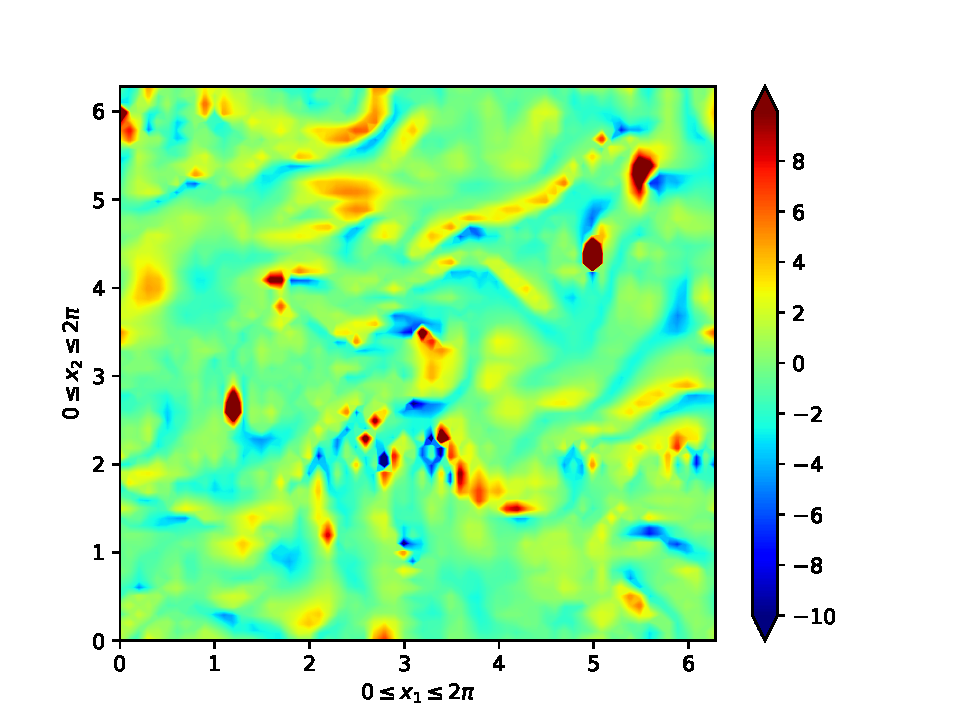
\includegraphics[height=1.75in]{media/run-cds-00/ke-RHS-CDS-00}
%        \caption{$\frac{1}{k} \frac{Dk}{Dt}$}
%    \end{subfigure}
%    ~
%    \begin{subfigure}[H]{0.45\textwidth}
%        \includegraphics[height=1.75in]{media/run-cds-00/enstrophy-RHS-CDS-00}
%        \caption{$\frac{1}{\Omega} \frac{D \Omega}{Dt}$}
%    \end{subfigure}
%    \newline
%    \begin{subfigure}{0.45\textwidth}
%        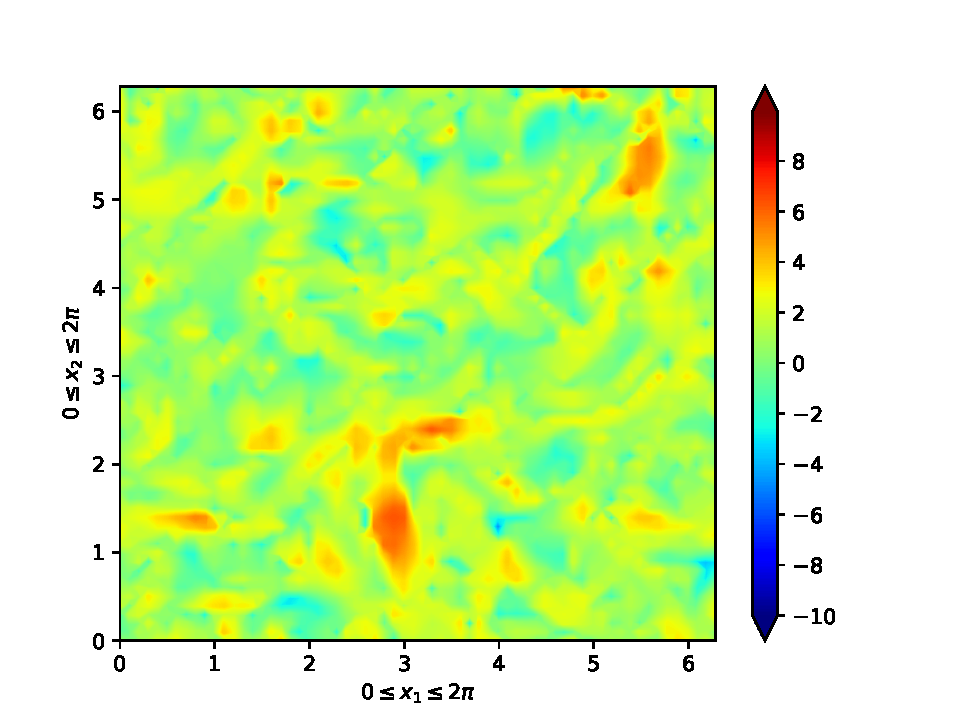
\includegraphics[height=1.75in]{media/run-cds-00/A-enst-CDS-00}
%        \caption{$A_{\Omega}$}
%    \end{subfigure}
%    ~
%    \begin{subfigure}{0.45\textwidth}
%        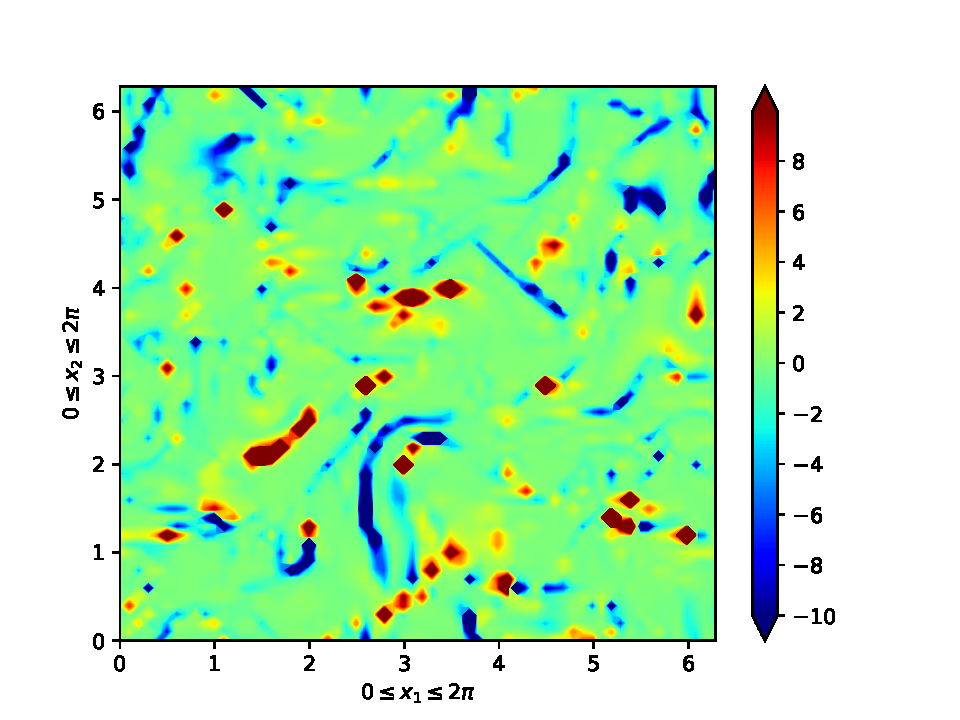
\includegraphics[height=1.75in]{media/run-cds-00/trans-enst-CDS-00}
%        \caption{$\Pi_{\Omega}$}
%    \end{subfigure}
%    \newline
%    \begin{subfigure}{0.45\textwidth}
%        \includegraphics[height=1.75in]{media/run-cds-00/prod-enst-CDS-00}
%        \caption{$P_{\Omega}$}
%    \end{subfigure}
%    ~
%    \begin{subfigure}{0.45\textwidth}
%        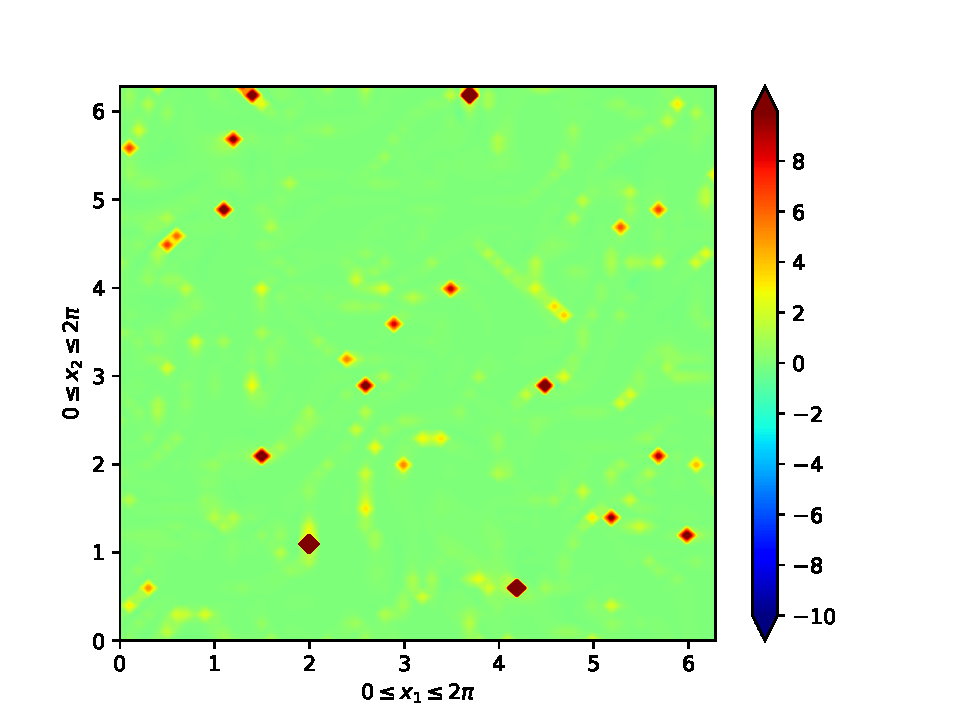
\includegraphics[height=1.75in]{media/run-cds-00/B-enst-CDS-00}
%        \caption{$B_{\Omega}$}
%    \end{subfigure}
%    \newline
%    \begin{subfigure}{0.45\textwidth}
%        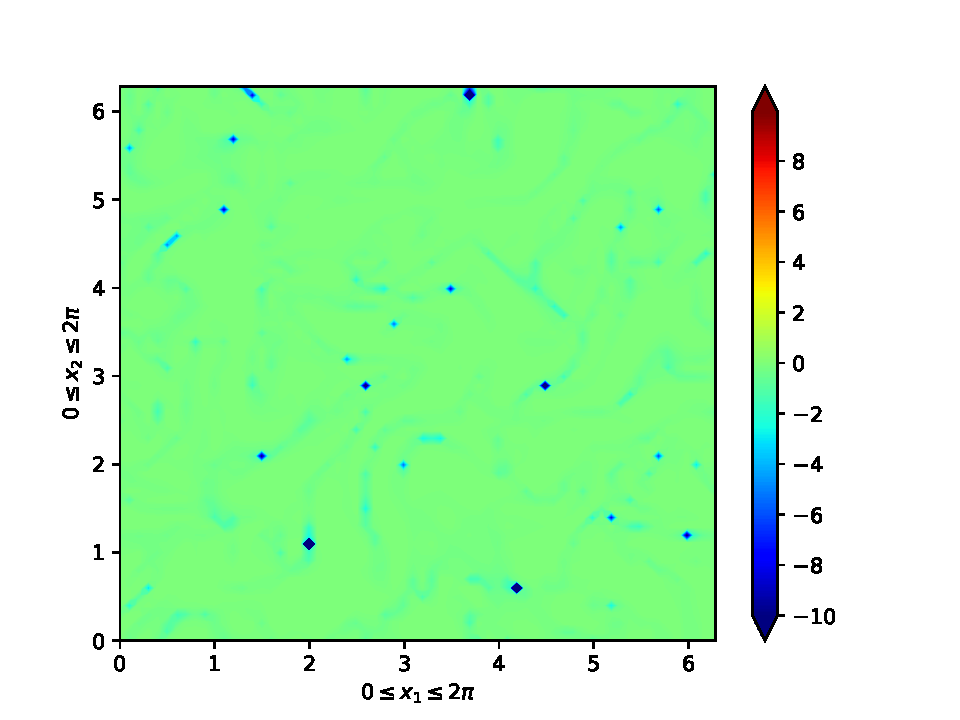
\includegraphics[height=1.75in]{media/run-cds-00/D-enst-CDS-00}
%        \caption{$D_{\Omega}$}
%    \end{subfigure}
%\end{figure}
%\newpage

%------------------------------------------------------------------------------%
% 1330                                                                         %
%------------------------------------------------------------------------------%
\begin{figure}[H]
    \begin{subfigure}[H]{0.45\textwidth}
        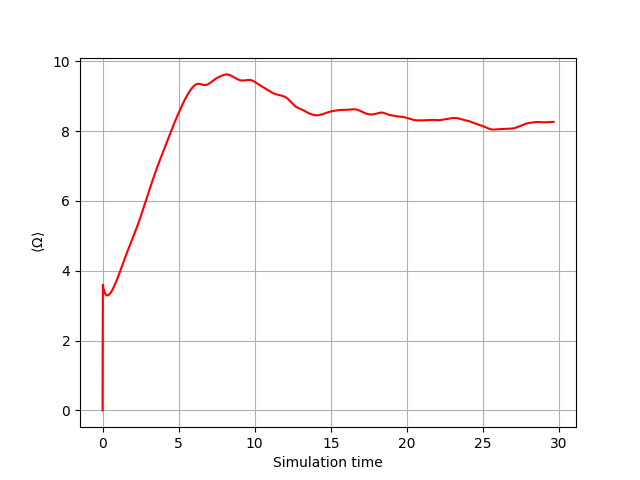
\includegraphics[height=1.75in]{media/run-cds-65/enst-average1330.png}
        \caption{Average enstrophy}
    \end{subfigure}
    ~
    \begin{subfigure}[H]{0.45\textwidth}
        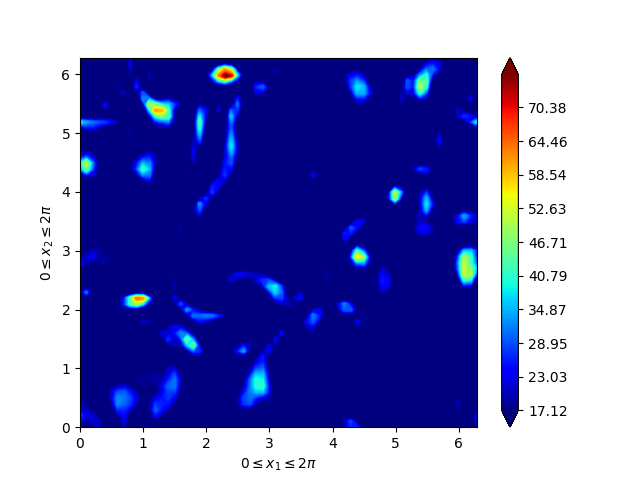
\includegraphics[height=1.75in]{media/run-cds-65/enst-2-1330.png}
        \caption{$[2\Omega_{rms}, \Omega_{max} ]$ }
    \end{subfigure}
    \newline
    \begin{subfigure}[H]{0.45\textwidth}
        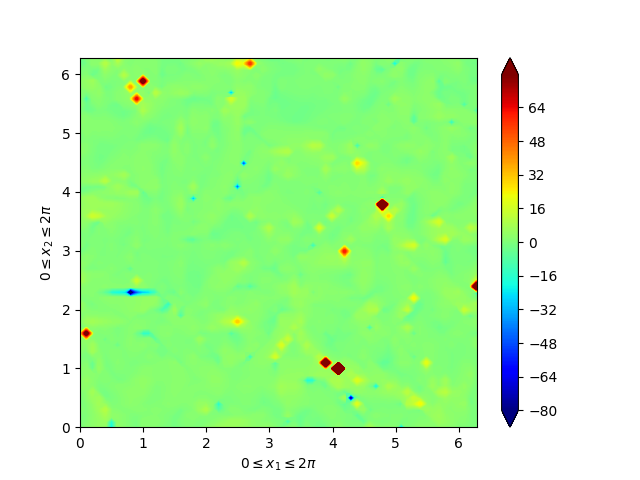
\includegraphics[height=1.75in]{media/run-cds-65/enst-1330.png}
        \caption{$\frac{1}{\Omega} \frac{D \Omega}{Dt}$}
    \end{subfigure}
    ~
    \begin{subfigure}{0.45\textwidth}
        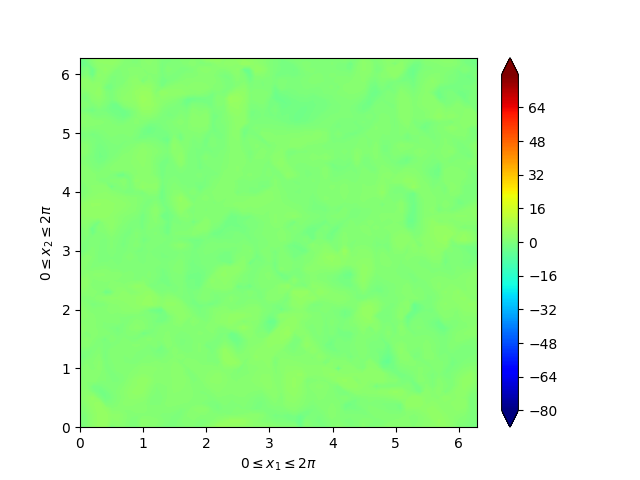
\includegraphics[height=1.75in]{media/run-cds-65/A-enst-1330.png}
        \caption{$A_{\Omega}$}
    \end{subfigure}
    \newline
    \begin{subfigure}{0.45\textwidth}
        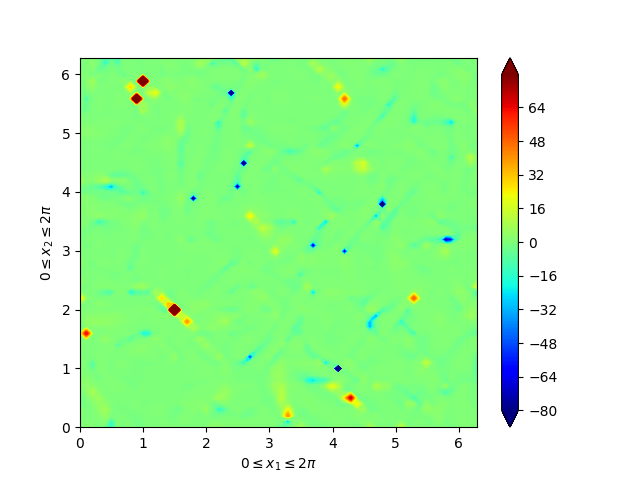
\includegraphics[height=1.75in]{media/run-cds-65/Pi-enst-1330.png}
        \caption{$\Pi_{\Omega}$}
    \end{subfigure}
    ~
    \begin{subfigure}{0.45\textwidth}
        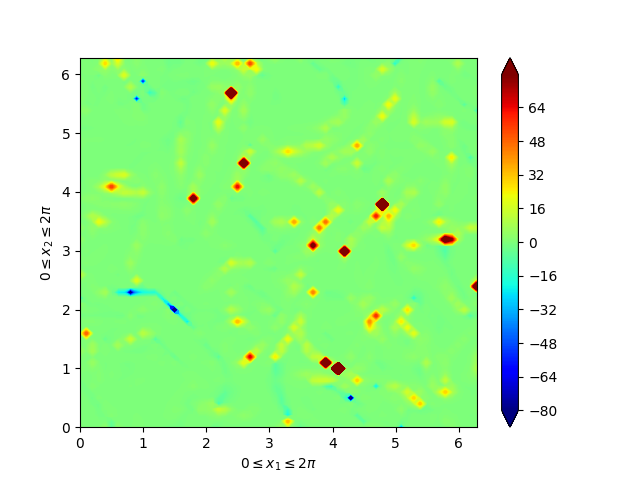
\includegraphics[height=1.75in]{media/run-cds-65/P-enst-1330.png}
        \caption{$P_{\Omega}$}
    \end{subfigure}
    \newline
    \begin{subfigure}{0.45\textwidth}
        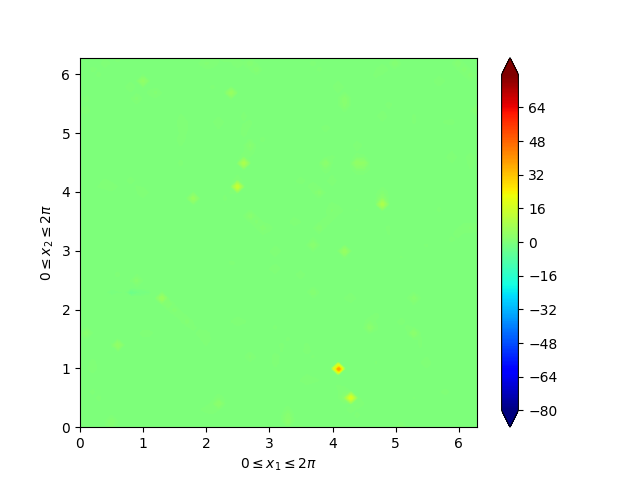
\includegraphics[height=1.75in]{media/run-cds-65/B-enst-1330.png}
        \caption{$B_{\Omega}$}
    \end{subfigure}
    ~
    \begin{subfigure}{0.45\textwidth}
        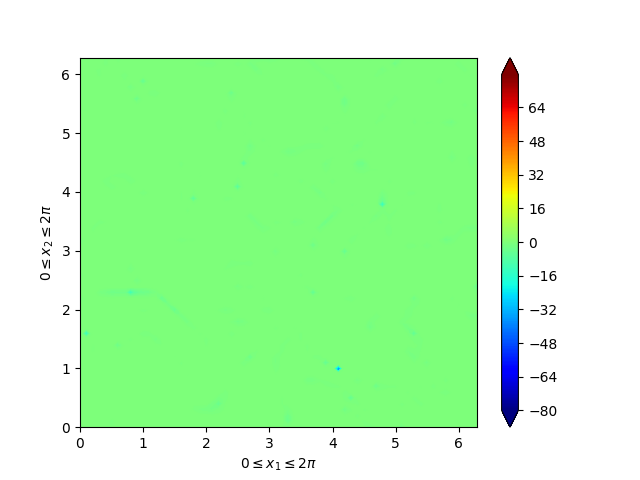
\includegraphics[height=1.75in]{media/run-cds-65/D-enst-1330.png}
        \caption{$D_{\Omega}$}
    \end{subfigure}
    \caption{Enstrophy transport terms for $t=29.65$, i.e., $t=t^{\ast} - 10 \Delta t$}
    \label{fig:enst-1330.png}
\end{figure}

\newpage

\begin{figure}[H]
    \begin{subfigure}[H]{0.45\textwidth}
        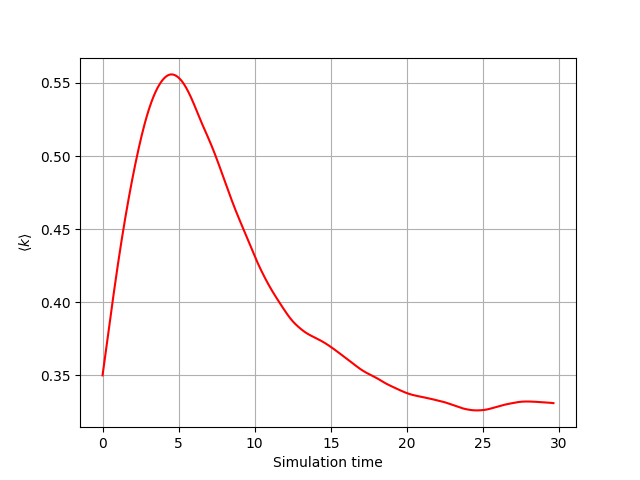
\includegraphics[height=1.75in]{media/run-cds-65/ke-average1330.png}
        \caption{Average kinetic energy}
    \end{subfigure}
    ~
    \begin{subfigure}[H]{0.45\textwidth}
        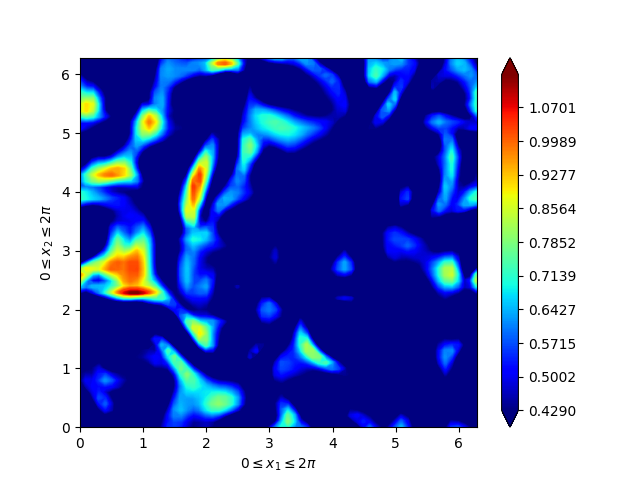
\includegraphics[height=1.75in]{media/run-cds-65/ke-2-1330.png}
        \caption{$[2k_{rms}, k_{max} $] }
    \end{subfigure}
    \newline
    \begin{subfigure}[H]{0.45\textwidth}
        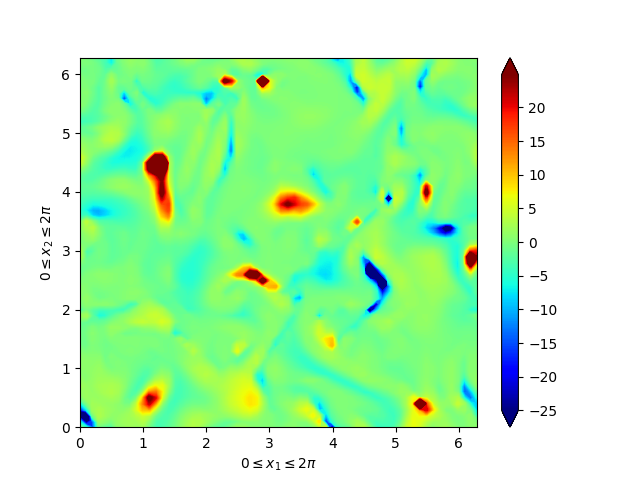
\includegraphics[height=1.75in]{media/run-cds-65/ke-1330.png}
        \caption{$\frac{1}{k} \frac{D k}{Dt}$}
    \end{subfigure}
    ~
    \begin{subfigure}{0.45\textwidth}
        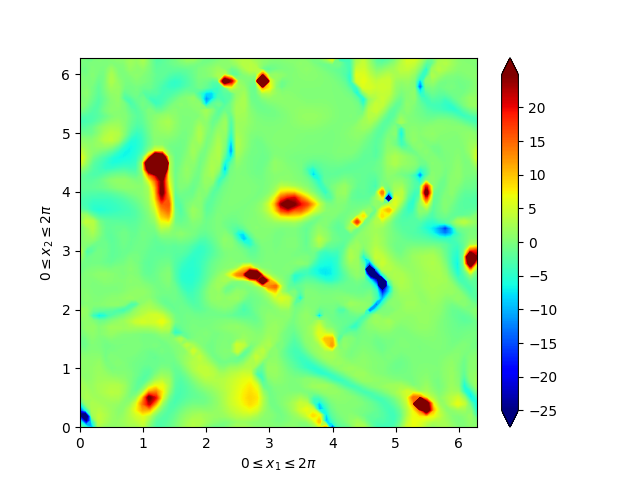
\includegraphics[height=1.75in]{media/run-cds-65/A-ke-1330.png}
        \caption{$A$}
    \end{subfigure}
    \newline
    \begin{subfigure}{0.45\textwidth}
        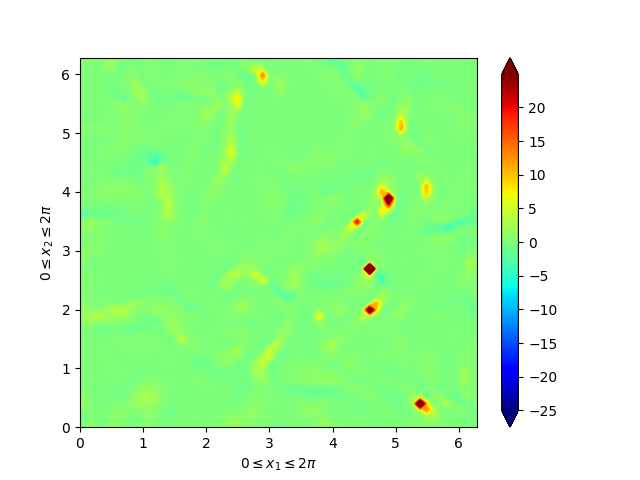
\includegraphics[height=1.75in]{media/run-cds-65/C-ke-1330.png}
        \caption{$C$}
    \end{subfigure}
    ~
    \begin{subfigure}{0.45\textwidth}
        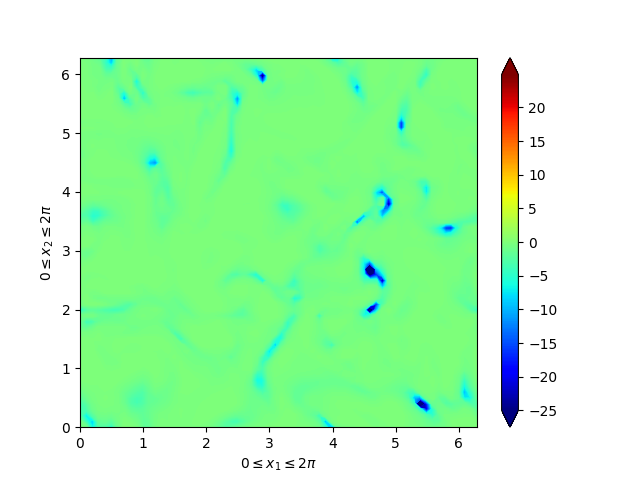
\includegraphics[height=1.75in]{media/run-cds-65/P-ke-1330.png}
        \caption{$P$}
    \end{subfigure}
    \newline
    \begin{subfigure}{0.45\textwidth}
        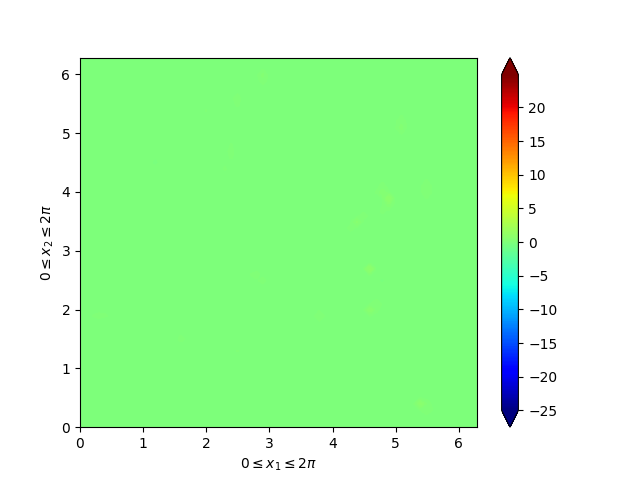
\includegraphics[height=1.75in]{media/run-cds-65/B-ke-1330.png}
        \caption{$B$}
    \end{subfigure}
    ~
    \begin{subfigure}{0.45\textwidth}
        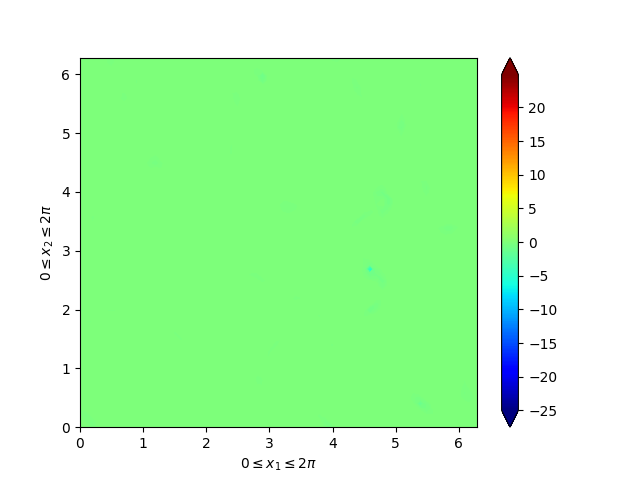
\includegraphics[height=1.75in]{media/run-cds-65/D-ke-1330.png}
        \caption{$D$}
    \end{subfigure}
    \caption{Kinetic energy transport terms for $t=29.65$, i.e., $t=t^{\ast} - 10 \Delta t$}
\end{figure}

\newpage

%------------------------------------------------------------------------------%
% 1335                                                                         %
%------------------------------------------------------------------------------%
\begin{figure}[H]
    \begin{subfigure}[H]{0.45\textwidth}
        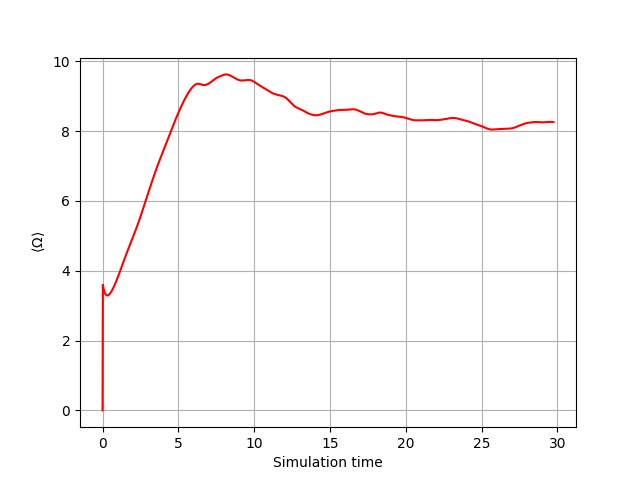
\includegraphics[height=1.75in]{media/run-cds-65/enst-average1335.png}
        \caption{Average enstrophy}
    \end{subfigure}
    ~
    \begin{subfigure}[H]{0.45\textwidth}
        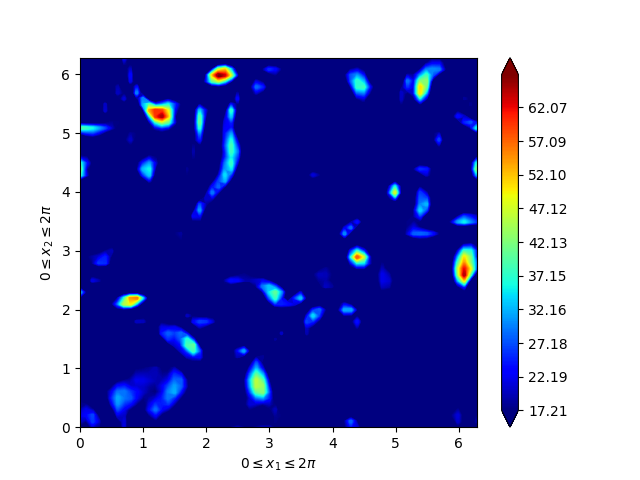
\includegraphics[height=1.75in]{media/run-cds-65/enst-2-1335.png}
        \caption{$[2\Omega_{rms}, \Omega_{max} $] }
    \end{subfigure}
    \newline
    \begin{subfigure}[H]{0.45\textwidth}
        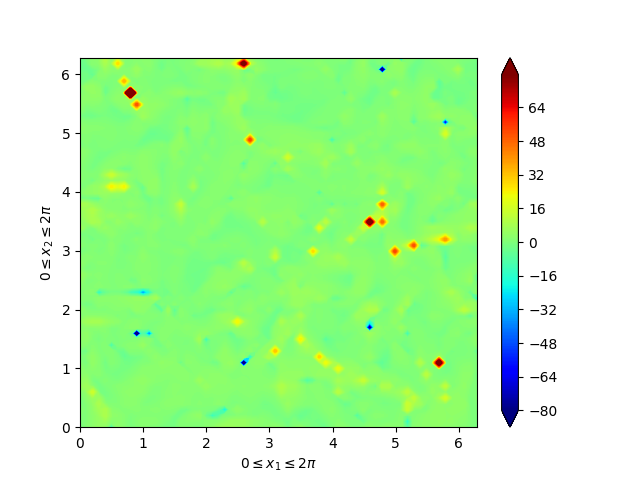
\includegraphics[height=1.75in]{media/run-cds-65/enst-1335.png}
        \caption{$\frac{1}{\Omega} \frac{D \Omega}{Dt}$}
    \end{subfigure}
    ~
    \begin{subfigure}{0.45\textwidth}
        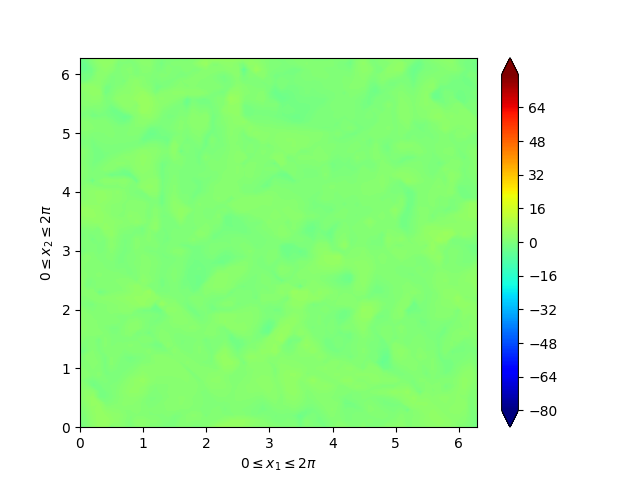
\includegraphics[height=1.75in]{media/run-cds-65/A-enst-1335.png}
        \caption{$A_{\Omega}$}
    \end{subfigure}
    \newline
    \begin{subfigure}{0.45\textwidth}
        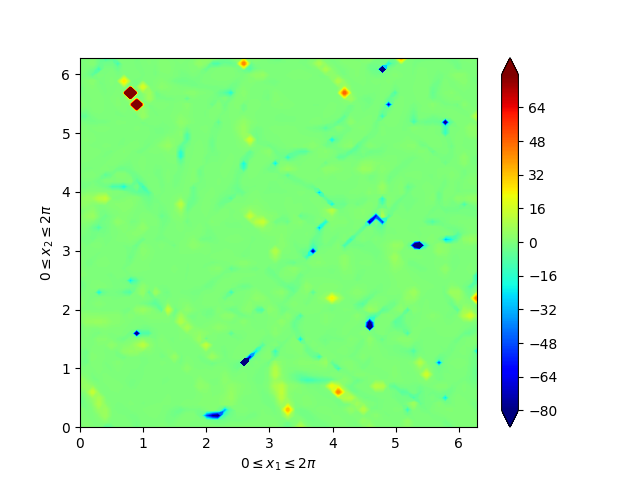
\includegraphics[height=1.75in]{media/run-cds-65/Pi-enst-1335.png}
        \caption{$\Pi_{\Omega}$}
    \end{subfigure}
    ~
    \begin{subfigure}{0.45\textwidth}
        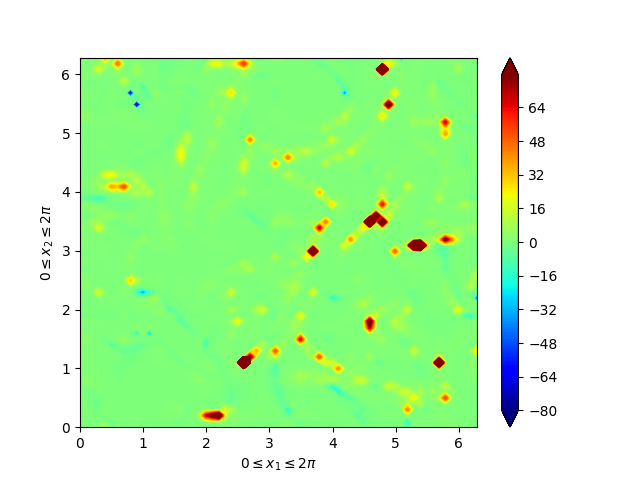
\includegraphics[height=1.75in]{media/run-cds-65/P-enst-1335.png}
        \caption{$P_{\Omega}$}
    \end{subfigure}
    \newline
    \begin{subfigure}{0.45\textwidth}
        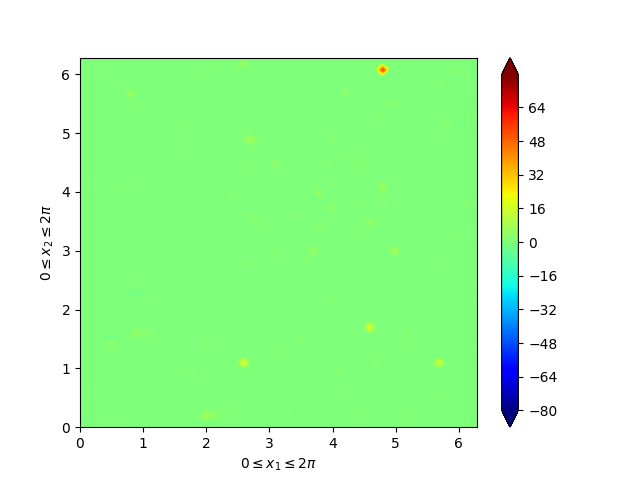
\includegraphics[height=1.75in]{media/run-cds-65/B-enst-1335.png}
        \caption{$B_{\Omega}$}
    \end{subfigure}
    ~
    \begin{subfigure}{0.45\textwidth}
        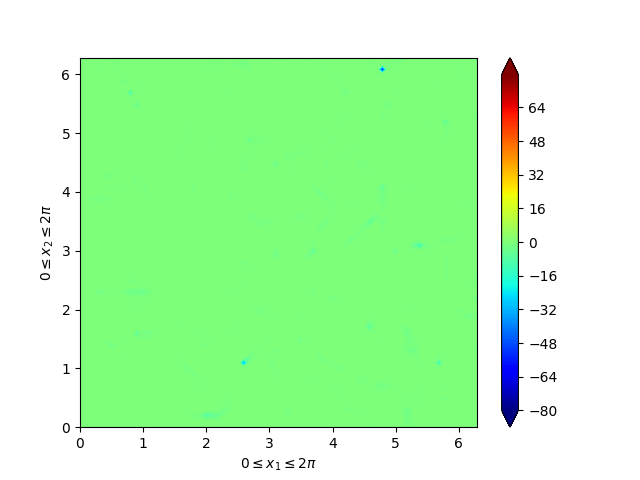
\includegraphics[height=1.75in]{media/run-cds-65/D-enst-1335.png}
        \caption{$D_{\Omega}$}
    \end{subfigure}
    \caption{Enstrophy transport terms for $t=29.77$, i.e., $t=t^{\ast} -5 \Delta t$}
\end{figure}

\newpage

\begin{figure}[H]
    \begin{subfigure}[H]{0.45\textwidth}
        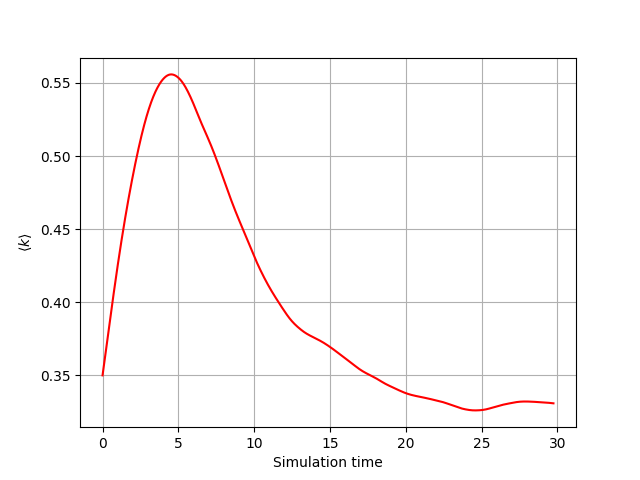
\includegraphics[height=1.75in]{media/run-cds-65/ke-average1335.png}
        \caption{Average kinetic energy}
    \end{subfigure}
    ~
    \begin{subfigure}[H]{0.45\textwidth}
        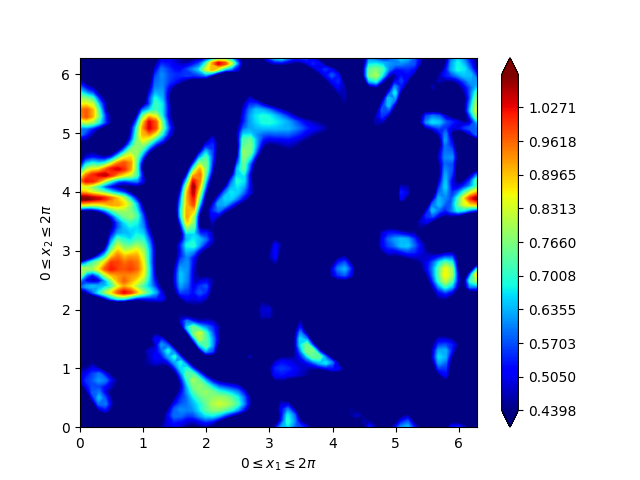
\includegraphics[height=1.75in]{media/run-cds-65/ke-2-1335.png}
        \caption{$[2k_{rms}, k_{max} $] }
    \end{subfigure}
    \newline
    \begin{subfigure}[H]{0.45\textwidth}
        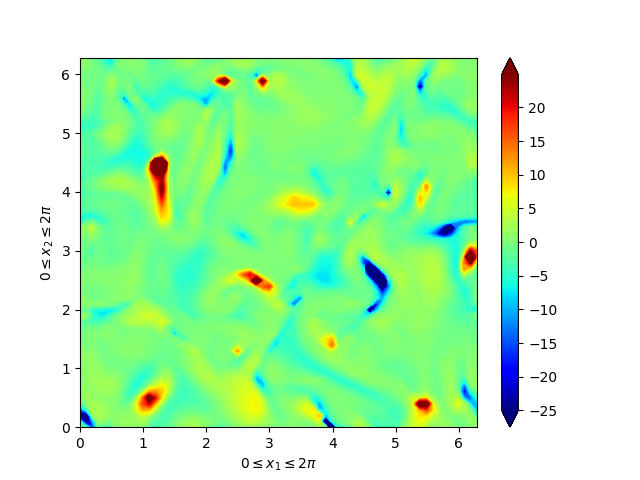
\includegraphics[height=1.75in]{media/run-cds-65/ke-1335.png}
        \caption{$\frac{1}{k} \frac{D k}{Dt}$}
    \end{subfigure}
    ~
    \begin{subfigure}{0.45\textwidth}
        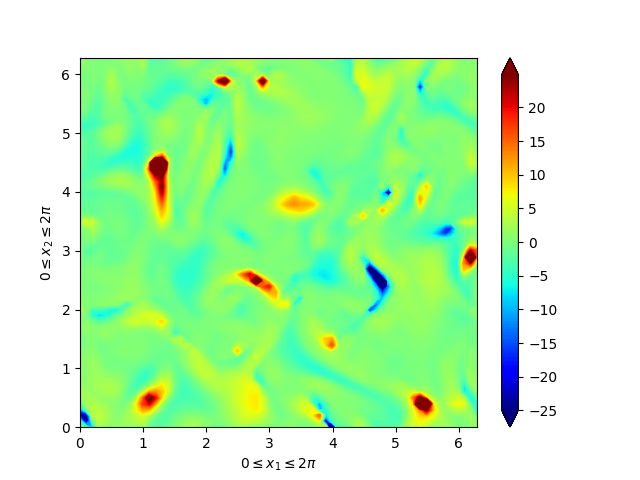
\includegraphics[height=1.75in]{media/run-cds-65/A-ke-1335.png}
        \caption{$A$}
    \end{subfigure}
    \newline
    \begin{subfigure}{0.45\textwidth}
        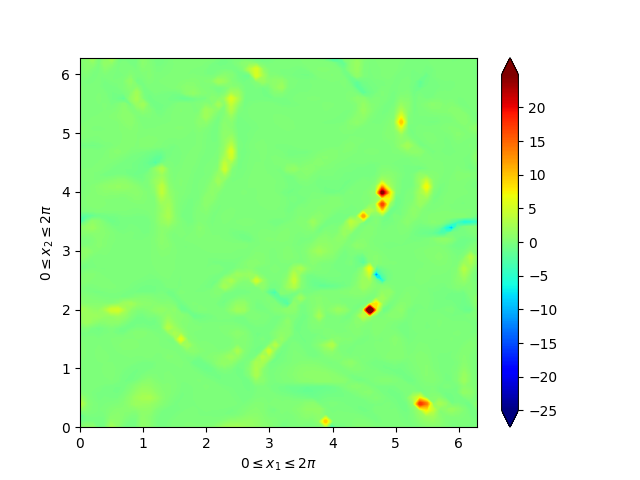
\includegraphics[height=1.75in]{media/run-cds-65/C-ke-1335.png}
        \caption{$C$}
    \end{subfigure}
    ~
    \begin{subfigure}{0.45\textwidth}
        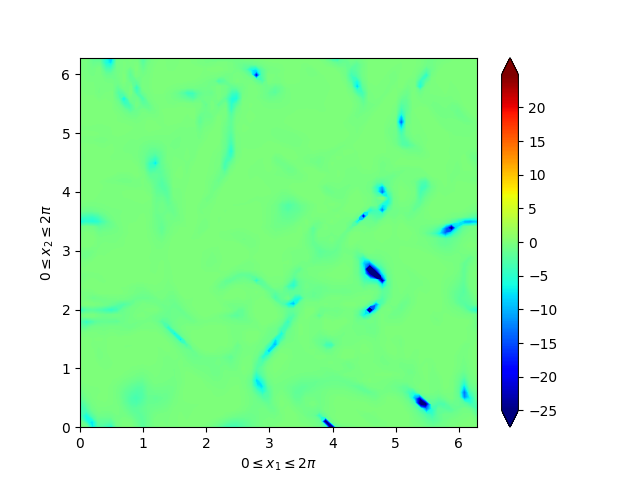
\includegraphics[height=1.75in]{media/run-cds-65/P-ke-1335.png}
        \caption{$P$}
    \end{subfigure}
    \newline
    \begin{subfigure}{0.45\textwidth}
        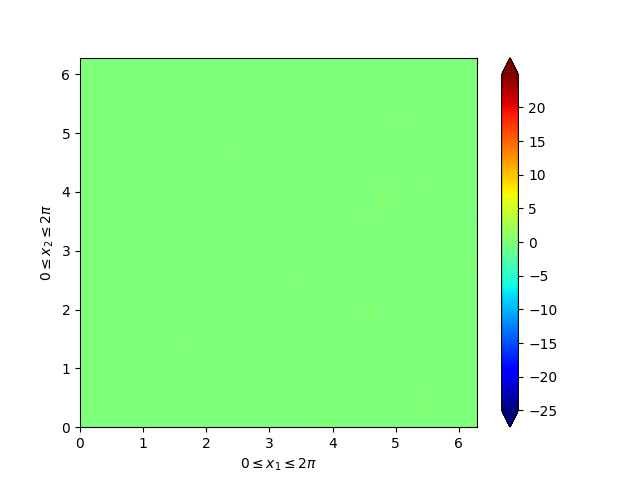
\includegraphics[height=1.75in]{media/run-cds-65/B-ke-1335.png}
        \caption{$B$}
    \end{subfigure}
    ~
    \begin{subfigure}{0.45\textwidth}
        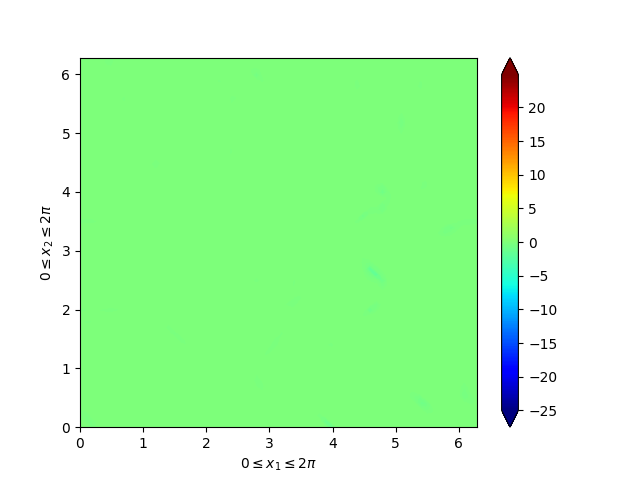
\includegraphics[height=1.75in]{media/run-cds-65/D-ke-1335.png}
        \caption{$D$}
    \end{subfigure}
    \caption{Kinetic energy transport terms for $t=29.77$, i.e., $t=t^{\ast} -5 \Delta t$}
\end{figure}

%------------------------------------------------------------------------------%
% 1340                                                                         %
%------------------------------------------------------------------------------%
\begin{figure}[H]
    \begin{subfigure}[H]{0.45\textwidth}
        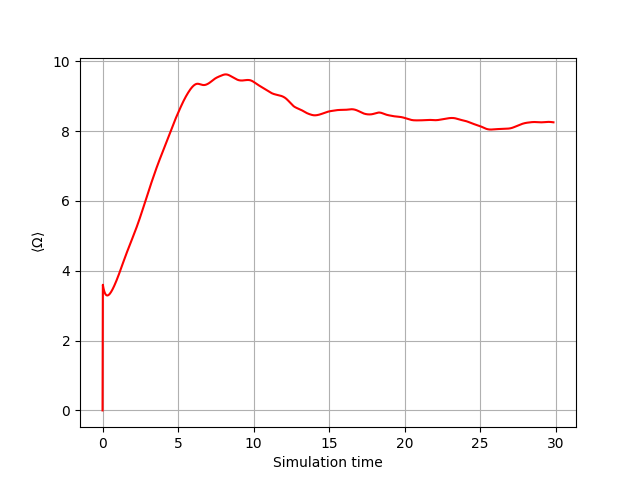
\includegraphics[height=1.75in]{media/run-cds-65/enst-average1340.png}
        \caption{Average enstrophy}
    \end{subfigure}
    ~
    \begin{subfigure}[H]{0.45\textwidth}
        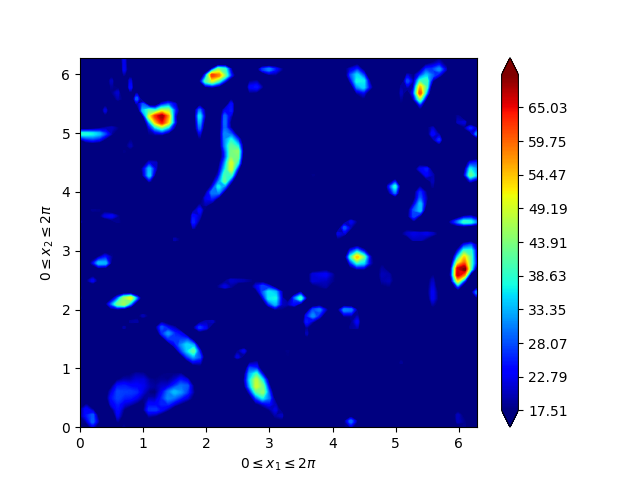
\includegraphics[height=1.75in]{media/run-cds-65/enst-2-1340.png}
        \caption{$[2\Omega_{rms}, \Omega_{max} $] }
    \end{subfigure}
    \newline
    \begin{subfigure}[H]{0.45\textwidth}
        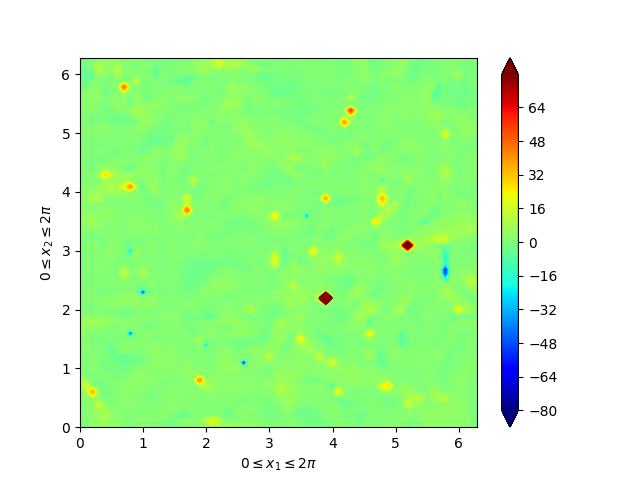
\includegraphics[height=1.75in]{media/run-cds-65/enst-1340.png}
        \caption{$\frac{1}{\Omega} \frac{D \Omega}{Dt}$}
    \end{subfigure}
    ~
    \begin{subfigure}{0.45\textwidth}
        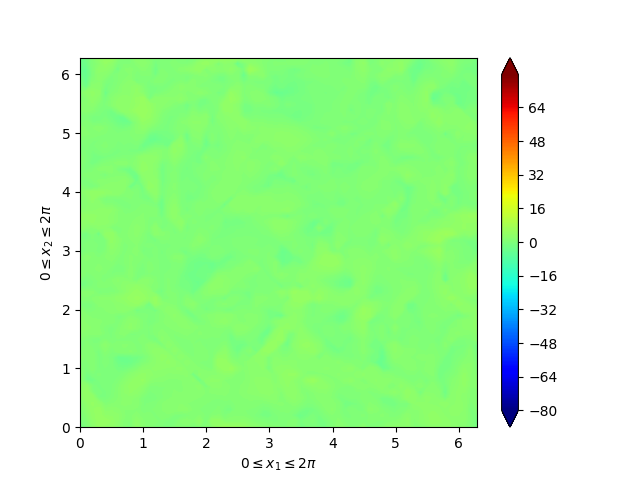
\includegraphics[height=1.75in]{media/run-cds-65/A-enst-1340.png}
        \caption{$A_{\Omega}$}
    \end{subfigure}
    \newline
    \begin{subfigure}{0.45\textwidth}
        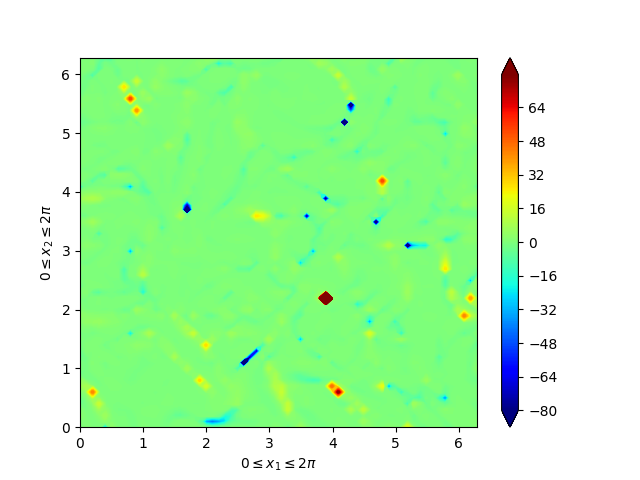
\includegraphics[height=1.75in]{media/run-cds-65/Pi-enst-1340.png}
        \caption{$\Pi_{\Omega}$}
    \end{subfigure}
    ~
    \begin{subfigure}{0.45\textwidth}
        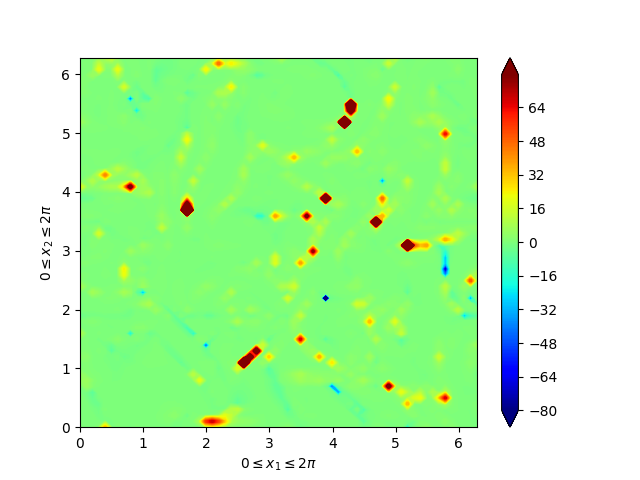
\includegraphics[height=1.75in]{media/run-cds-65/P-enst-1340.png}
        \caption{$P_{\Omega}$}
    \end{subfigure}
    \newline
    \begin{subfigure}{0.45\textwidth}
        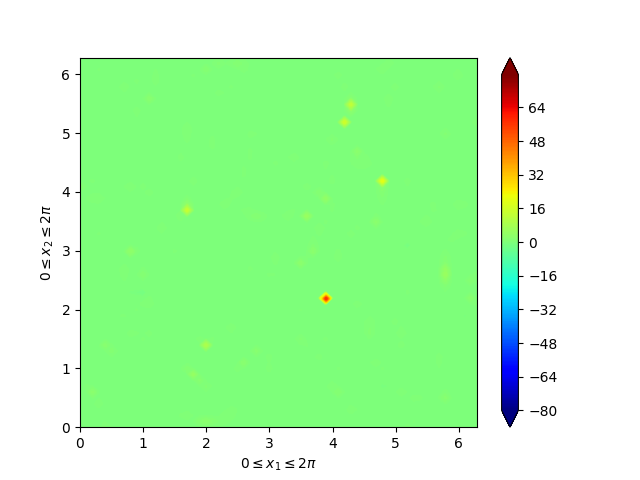
\includegraphics[height=1.75in]{media/run-cds-65/B-enst-1340.png}
        \caption{$B_{\Omega}$}
    \end{subfigure}
    ~
    \begin{subfigure}{0.45\textwidth}
        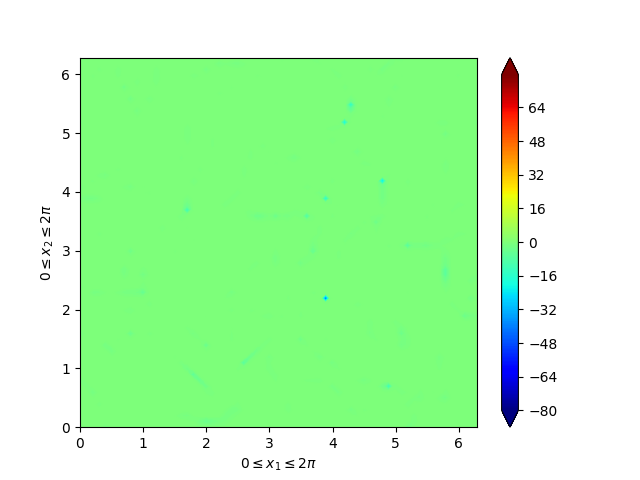
\includegraphics[height=1.75in]{media/run-cds-65/D-enst-1340.png}
        \caption{$D_{\Omega}$}
    \end{subfigure}
    \caption{Enstrophy transport terms for $t=30.01$, i.e., $t=t^{\ast} $}
\end{figure}

\newpage

\begin{figure}[H]
    \begin{subfigure}[H]{0.45\textwidth}
        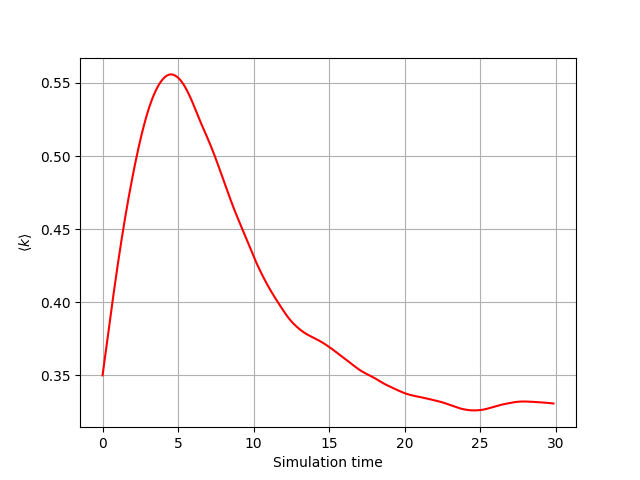
\includegraphics[height=1.75in]{media/run-cds-65/ke-average1340.png}
        \caption{Average kinetic energy}
    \end{subfigure}
    ~
    \begin{subfigure}[H]{0.45\textwidth}
        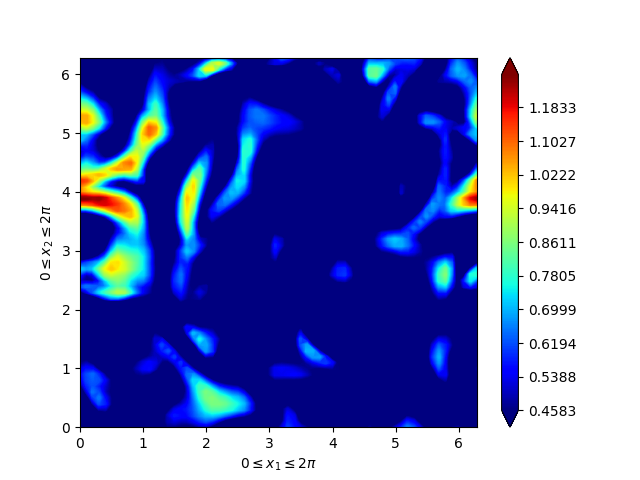
\includegraphics[height=1.75in]{media/run-cds-65/ke-2-1340.png}
        \caption{$[2k_{rms}, k_{max} $] }
    \end{subfigure}
    \newline
    \begin{subfigure}[H]{0.45\textwidth}
        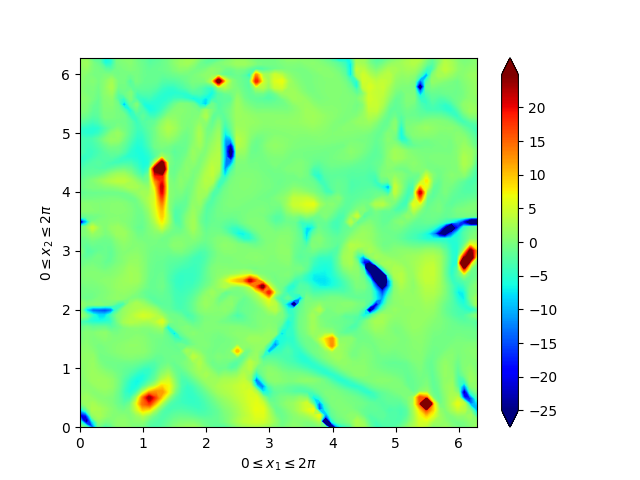
\includegraphics[height=1.75in]{media/run-cds-65/ke-1340.png}
        \caption{$\frac{1}{k} \frac{D k}{Dt}$}
    \end{subfigure}
    ~
    \begin{subfigure}{0.45\textwidth}
        \includegraphics[height=1.75in]{media/run-cds-65/A-ke-1340.png}
        \caption{$A$}
    \end{subfigure}
    \newline
    \begin{subfigure}{0.45\textwidth}
        \includegraphics[height=1.75in]{media/run-cds-65/C-ke-1340.png}
        \caption{$C$}
    \end{subfigure}
    ~
    \begin{subfigure}{0.45\textwidth}
        \includegraphics[height=1.75in]{media/run-cds-65/P-ke-1340.png}
        \caption{$P$}
    \end{subfigure}
    \newline
    \begin{subfigure}{0.45\textwidth}
        \includegraphics[height=1.75in]{media/run-cds-65/B-ke-1340.png}
        \caption{$B$}
    \end{subfigure}
    ~
    \begin{subfigure}{0.45\textwidth}
        \includegraphics[height=1.75in]{media/run-cds-65/D-ke-1340.png}
        \caption{$D$}
    \end{subfigure}
    \caption{Kinetic energy transport terms for $t=30.01$, i.e., $t=t^{\ast} $}
\end{figure}
%------------------------------------------------------------------------------%
% 1360                                                                         %
%------------------------------------------------------------------------------%
\begin{figure}[H]
    \begin{subfigure}[H]{0.45\textwidth}
        \includegraphics[height=1.75in]{media/run-cds-65/enst-average1360.png}
        \caption{Average enstrophy}
    \end{subfigure}
    ~
    \begin{subfigure}[H]{0.45\textwidth}
        \includegraphics[height=1.75in]{media/run-cds-65/enst-2-1360.png}
        \caption{$[2\Omega_{rms}, \Omega_{max} $] }
    \end{subfigure}
    \newline
    \begin{subfigure}[H]{0.45\textwidth}
        \includegraphics[height=1.75in]{media/run-cds-65/enst-1360.png}
        \caption{$\frac{1}{\Omega} \frac{D \Omega}{Dt}$}
    \end{subfigure}
    ~
    \begin{subfigure}{0.45\textwidth}
        \includegraphics[height=1.75in]{media/run-cds-65/A-enst-1360.png}
        \caption{$A_{\Omega}$}
    \end{subfigure}
    \newline
    \begin{subfigure}{0.45\textwidth}
        \includegraphics[height=1.75in]{media/run-cds-65/Pi-enst-1360.png}
        \caption{$\Pi_{\Omega}$}
    \end{subfigure}
    ~
    \begin{subfigure}{0.45\textwidth}
        \includegraphics[height=1.75in]{media/run-cds-65/P-enst-1360.png}
        \caption{$P_{\Omega}$}
    \end{subfigure}
    \newline
    \begin{subfigure}{0.45\textwidth}
        \includegraphics[height=1.75in]{media/run-cds-65/B-enst-1360.png}
        \caption{$B_{\Omega}$}
    \end{subfigure}
    ~
    \begin{subfigure}{0.45\textwidth}
        \includegraphics[height=1.75in]{media/run-cds-65/D-enst-1360.png}
        \caption{$D_{\Omega}$}
    \end{subfigure}
    \caption{Enstrophy transport terms for $t=30.32$, i.e., $t=t^{\ast} + 20 \Delta t$}
\end{figure}

\newpage

\begin{figure}[H]
    \begin{subfigure}[H]{0.45\textwidth}
        \includegraphics[height=1.75in]{media/run-cds-65/ke-average1360.png}
        \caption{Average kinetic energy}
    \end{subfigure}
    ~
    \begin{subfigure}[H]{0.45\textwidth}
        \includegraphics[height=1.75in]{media/run-cds-65/ke-2-1360.png}
        \caption{$[2k_{rms}, k_{max} $] }
    \end{subfigure}
    \newline
    \begin{subfigure}[H]{0.45\textwidth}
        \includegraphics[height=1.75in]{media/run-cds-65/ke-1360.png}
        \caption{$\frac{1}{k} \frac{D k}{Dt}$}
    \end{subfigure}
    ~
    \begin{subfigure}{0.45\textwidth}
        \includegraphics[height=1.75in]{media/run-cds-65/A-ke-1360.png}
        \caption{$A$}
    \end{subfigure}
    \newline
    \begin{subfigure}{0.45\textwidth}
        \includegraphics[height=1.75in]{media/run-cds-65/C-ke-1360.png}
        \caption{$C$}
    \end{subfigure}
    ~
    \begin{subfigure}{0.45\textwidth}
        \includegraphics[height=1.75in]{media/run-cds-65/P-ke-1360.png}
        \caption{$P$}
    \end{subfigure}
    \newline
    \begin{subfigure}{0.45\textwidth}
        \includegraphics[height=1.75in]{media/run-cds-65/B-ke-1360.png}
        \caption{$B$}
    \end{subfigure}
    ~
    \begin{subfigure}{0.45\textwidth}
        \includegraphics[height=1.75in]{media/run-cds-65/D-ke-1360.png}
        \caption{$D$}
    \end{subfigure}
    \caption{Kinetic energy transport terms for $t=30.32$, i.e., $t=t^{\ast} + 20 \Delta t$}
\end{figure}

%------------------------------------------------------------------------------%
% 1380                                                                         %
%------------------------------------------------------------------------------%
\begin{figure}[H]
    \begin{subfigure}[H]{0.45\textwidth}
        \includegraphics[height=1.75in]{media/run-cds-65/enst-average1380.png}
        \caption{Average enstrophy}
    \end{subfigure}
    ~
    \begin{subfigure}[H]{0.45\textwidth}
        \includegraphics[height=1.75in]{media/run-cds-65/enst-2-1380.png}
        \caption{$[2\Omega_{rms}, \Omega_{max} $] }
    \end{subfigure}
    \newline
    \begin{subfigure}[H]{0.45\textwidth}
        \includegraphics[height=1.75in]{media/run-cds-65/enst-1380.png}
        \caption{$\frac{1}{\Omega} \frac{D \Omega}{Dt}$}
    \end{subfigure}
    ~
    \begin{subfigure}{0.45\textwidth}
        \includegraphics[height=1.75in]{media/run-cds-65/A-enst-1380.png}
        \caption{$A_{\Omega}$}
    \end{subfigure}
    \newline
    \begin{subfigure}{0.45\textwidth}
        \includegraphics[height=1.75in]{media/run-cds-65/Pi-enst-1380.png}
        \caption{$\Pi_{\Omega}$}
    \end{subfigure}
    ~
    \begin{subfigure}{0.45\textwidth}
        \includegraphics[height=1.75in]{media/run-cds-65/P-enst-1380.png}
        \caption{$P_{\Omega}$}
    \end{subfigure}
    \newline
    \begin{subfigure}{0.45\textwidth}
        \includegraphics[height=1.75in]{media/run-cds-65/B-enst-1380.png}
        \caption{$B_{\Omega}$}
    \end{subfigure}
    ~
    \begin{subfigure}{0.45\textwidth}
        \includegraphics[height=1.75in]{media/run-cds-65/D-enst-1380.png}
        \caption{$D_{\Omega}$}
    \end{subfigure}
    \caption{Enstrophy transport terms for $t=30.67$, i.e., $t=t^{\ast} + 40 \Delta t$}
\end{figure}

\newpage

\begin{figure}[H]
    \begin{subfigure}[H]{0.45\textwidth}
        \includegraphics[height=1.75in]{media/run-cds-65/ke-average1380.png}
        \caption{Average kinetic energy}
    \end{subfigure}
    ~
    \begin{subfigure}[H]{0.45\textwidth}
        \includegraphics[height=1.75in]{media/run-cds-65/ke-2-1380.png}
        \caption{$[2k_{rms}, k_{max} $] }
    \end{subfigure}
    \newline
    \begin{subfigure}[H]{0.45\textwidth}
        \includegraphics[height=1.75in]{media/run-cds-65/ke-1380.png}
        \caption{$\frac{1}{k} \frac{D k}{Dt}$}
    \end{subfigure}
    ~
    \begin{subfigure}{0.45\textwidth}
        \includegraphics[height=1.75in]{media/run-cds-65/A-ke-1380.png}
        \caption{$A$}
    \end{subfigure}
    \newline
    \begin{subfigure}{0.45\textwidth}
        \includegraphics[height=1.75in]{media/run-cds-65/C-ke-1380.png}
        \caption{$C$}
    \end{subfigure}
    ~
    \begin{subfigure}{0.45\textwidth}
        \includegraphics[height=1.75in]{media/run-cds-65/P-ke-1380.png}
        \caption{$P$}
    \end{subfigure}
    \newline
    \begin{subfigure}{0.45\textwidth}
        \includegraphics[height=1.75in]{media/run-cds-65/B-ke-1380.png}
        \caption{$B$}
    \end{subfigure}
    ~
    \begin{subfigure}{0.45\textwidth}
        \includegraphics[height=1.75in]{media/run-cds-65/D-ke-1380.png}
        \caption{$D$}
    \end{subfigure}
    \caption{Kinetic energy transport terms for $t=30.67$, i.e., $t=t^{\ast} + 40 \Delta t$}
\end{figure}
%------------------------------------------------------------------------------%
% 1400                                                                         %
%------------------------------------------------------------------------------%
\begin{figure}[H]
    \begin{subfigure}[H]{0.45\textwidth}
        \includegraphics[height=1.75in]{media/run-cds-65/enst-average1400.png}
        \caption{Average enstrophy}
    \end{subfigure}
    ~
    \begin{subfigure}[H]{0.45\textwidth}
        \includegraphics[height=1.75in]{media/run-cds-65/enst-2-1400.png}
        \caption{$[2\Omega_{rms}, \Omega_{max} $] }
    \end{subfigure}
    \newline
    \begin{subfigure}[H]{0.45\textwidth}
        \includegraphics[height=1.75in]{media/run-cds-65/enst-1400.png}
        \caption{$\frac{1}{\Omega} \frac{D \Omega}{Dt}$}
    \end{subfigure}
    ~
    \begin{subfigure}{0.45\textwidth}
        \includegraphics[height=1.75in]{media/run-cds-65/A-enst-1400.png}
        \caption{$A_{\Omega}$}
    \end{subfigure}
    \newline
    \begin{subfigure}{0.45\textwidth}
        \includegraphics[height=1.75in]{media/run-cds-65/Pi-enst-1400.png}
        \caption{$\Pi_{\Omega}$}
    \end{subfigure}
    ~
    \begin{subfigure}{0.45\textwidth}
        \includegraphics[height=1.75in]{media/run-cds-65/P-enst-1400.png}
        \caption{$P_{\Omega}$}
    \end{subfigure}
    \newline
    \begin{subfigure}{0.45\textwidth}
        \includegraphics[height=1.75in]{media/run-cds-65/B-enst-1400.png}
        \caption{$B_{\Omega}$}
    \end{subfigure}
    ~
    \begin{subfigure}{0.45\textwidth}
        \includegraphics[height=1.75in]{media/run-cds-65/D-enst-1400.png}
        \caption{$D_{\Omega}$}
    \end{subfigure}
    \caption{Enstrophy transport terms for $t=30.80$, i.e., $t=t^{\ast} + 60 \Delta t$}
\end{figure}

\newpage

\begin{figure}[H]
    \begin{subfigure}[H]{0.45\textwidth}
        \includegraphics[height=1.75in]{media/run-cds-65/ke-average1400.png}
        \caption{Average kinetic energy}
    \end{subfigure}
    ~
    \begin{subfigure}[H]{0.45\textwidth}
        \includegraphics[height=1.75in]{media/run-cds-65/ke-2-1400.png}
        \caption{$[2k_{rms}, k_{max} $] }
    \end{subfigure}
    \newline
    \begin{subfigure}[H]{0.45\textwidth}
        \includegraphics[height=1.75in]{media/run-cds-65/ke-1400.png}
        \caption{$\frac{1}{k} \frac{D k}{Dt}$}
    \end{subfigure}
    ~
    \begin{subfigure}{0.45\textwidth}
        \includegraphics[height=1.75in]{media/run-cds-65/A-ke-1400.png}
        \caption{$A$}
    \end{subfigure}
    \newline
    \begin{subfigure}{0.45\textwidth}
        \includegraphics[height=1.75in]{media/run-cds-65/C-ke-1400.png}
        \caption{$C$}
    \end{subfigure}
    ~
    \begin{subfigure}{0.45\textwidth}
        \includegraphics[height=1.75in]{media/run-cds-65/P-ke-1400.png}
        \caption{$P$}
    \end{subfigure}
    \newline
    \begin{subfigure}{0.45\textwidth}
        \includegraphics[height=1.75in]{media/run-cds-65/B-ke-1400.png}
        \caption{$B$}
    \end{subfigure}
    ~
    \begin{subfigure}{0.45\textwidth}
        \includegraphics[height=1.75in]{media/run-cds-65/D-ke-1400.png}
        \caption{$D$}
    \end{subfigure}
    \caption{Kinetic energy transport terms for $t=30.80$, i.e., $t=t^{\ast} + 60 \Delta t$}
\end{figure}
%------------------------------------------------------------------------------%
% 1420                                                                         %
%------------------------------------------------------------------------------%
\begin{figure}[H]
    \begin{subfigure}[H]{0.45\textwidth}
        \includegraphics[height=1.75in]{media/run-cds-65/enst-average1420.png}
        \caption{Average enstrophy}
    \end{subfigure}
    ~
    \begin{subfigure}[H]{0.45\textwidth}
        \includegraphics[height=1.75in]{media/run-cds-65/enst-2-1420.png}
        \caption{$[2\Omega_{rms}, \Omega_{max} $] }
    \end{subfigure}
    \newline
    \begin{subfigure}[H]{0.45\textwidth}
        \includegraphics[height=1.75in]{media/run-cds-65/enst-1420.png}
        \caption{$\frac{1}{\Omega} \frac{D \Omega}{Dt}$}
    \end{subfigure}
    ~
    \begin{subfigure}{0.45\textwidth}
        \includegraphics[height=1.75in]{media/run-cds-65/A-enst-1420.png}
        \caption{$A_{\Omega}$}
    \end{subfigure}
    \newline
    \begin{subfigure}{0.45\textwidth}
        \includegraphics[height=1.75in]{media/run-cds-65/Pi-enst-1420.png}
        \caption{$\Pi_{\Omega}$}
    \end{subfigure}
    ~
    \begin{subfigure}{0.45\textwidth}
        \includegraphics[height=1.75in]{media/run-cds-65/P-enst-1420.png}
        \caption{$P_{\Omega}$}
    \end{subfigure}
    \newline
    \begin{subfigure}{0.45\textwidth}
        \includegraphics[height=1.75in]{media/run-cds-65/B-enst-1420.png}
        \caption{$B_{\Omega}$}
    \end{subfigure}
    ~
    \begin{subfigure}{0.45\textwidth}
        \includegraphics[height=1.75in]{media/run-cds-65/D-enst-1420.png}
        \caption{$D_{\Omega}$}
    \end{subfigure}
    \caption{Enstrophy transport terms for $t=30.88$, i.e., $t=t^{\ast} + 80 \Delta t$}
\end{figure}

\newpage

\begin{figure}[H]
    \begin{subfigure}[H]{0.45\textwidth}
        \includegraphics[height=1.75in]{media/run-cds-65/ke-average1420.png}
        \caption{Average kinetic energy}
    \end{subfigure}
    ~
    \begin{subfigure}[H]{0.45\textwidth}
        \includegraphics[height=1.75in]{media/run-cds-65/ke-2-1420.png}
        \caption{$[2k_{rms}, k_{max} $] }
    \end{subfigure}
    \newline
    \begin{subfigure}[H]{0.45\textwidth}
        \includegraphics[height=1.75in]{media/run-cds-65/ke-1420.png}
        \caption{$\frac{1}{k} \frac{D k}{Dt}$}
    \end{subfigure}
    ~
    \begin{subfigure}{0.45\textwidth}
        \includegraphics[height=1.75in]{media/run-cds-65/A-ke-1420.png}
        \caption{$A$}
    \end{subfigure}
    \newline
    \begin{subfigure}{0.45\textwidth}
        \includegraphics[height=1.75in]{media/run-cds-65/C-ke-1420.png}
        \caption{$C$}
    \end{subfigure}
    ~
    \begin{subfigure}{0.45\textwidth}
        \includegraphics[height=1.75in]{media/run-cds-65/P-ke-1420.png}
        \caption{$P$}
    \end{subfigure}
    \newline
    \begin{subfigure}{0.45\textwidth}
        \includegraphics[height=1.75in]{media/run-cds-65/B-ke-1420.png}
        \caption{$B$}
    \end{subfigure}
    ~
    \begin{subfigure}{0.45\textwidth}
        \includegraphics[height=1.75in]{media/run-cds-65/D-ke-1420.png}
        \caption{$D$}
    \end{subfigure}
    \caption{Kinetic energy transport terms for $t=30.88$, i.e., $t=t^{\ast} + 80 \Delta t$}
\end{figure}
%------------------------------------------------------------------------------%
% 1440                                                                         %
%------------------------------------------------------------------------------%
\begin{figure}[H]
    \begin{subfigure}[H]{0.45\textwidth}
        \includegraphics[height=1.75in]{media/run-cds-65/enst-average1440.png}
        \caption{Average enstrophy}
    \end{subfigure}
    ~
    \begin{subfigure}[H]{0.45\textwidth}
        \includegraphics[height=1.75in]{media/run-cds-65/enst-2-1440.png}
        \caption{$[2\Omega_{rms}, \Omega_{max} $] }
    \end{subfigure}
    \newline
    \begin{subfigure}[H]{0.45\textwidth}
        \includegraphics[height=1.75in]{media/run-cds-65/enst-1440.png}
        \caption{$\frac{1}{\Omega} \frac{D \Omega}{Dt}$}
    \end{subfigure}
    ~
    \begin{subfigure}{0.45\textwidth}
        \includegraphics[height=1.75in]{media/run-cds-65/A-enst-1440.png}
        \caption{$A_{\Omega}$}
    \end{subfigure}
    \newline
    \begin{subfigure}{0.45\textwidth}
        \includegraphics[height=1.75in]{media/run-cds-65/Pi-enst-1440.png}
        \caption{$\Pi_{\Omega}$}
    \end{subfigure}
    ~
    \begin{subfigure}{0.45\textwidth}
        \includegraphics[height=1.75in]{media/run-cds-65/P-enst-1440.png}
        \caption{$P_{\Omega}$}
    \end{subfigure}
    \newline
    \begin{subfigure}{0.45\textwidth}
        \includegraphics[height=1.75in]{media/run-cds-65/B-enst-1440.png}
        \caption{$B_{\Omega}$}
    \end{subfigure}
    ~
    \begin{subfigure}{0.45\textwidth}
        \includegraphics[height=1.75in]{media/run-cds-65/D-enst-1440.png}
        \caption{$D_{\Omega}$}
    \end{subfigure}
    \caption{Enstrophy transport terms for $t=30.93$, i.e., $t=t^{\ast} + 100 \Delta t$}
\end{figure}

\newpage

\begin{figure}[H]
    \begin{subfigure}[H]{0.45\textwidth}
        \includegraphics[height=1.75in]{media/run-cds-65/ke-average1440.png}
        \caption{Average kinetic energy}
    \end{subfigure}
    ~
    \begin{subfigure}[H]{0.45\textwidth}
        \includegraphics[height=1.75in]{media/run-cds-65/ke-2-1440.png}
        \caption{$[2k_{rms}, k_{max} $] }
    \end{subfigure}
    \newline
    \begin{subfigure}[H]{0.45\textwidth}
        \includegraphics[height=1.75in]{media/run-cds-65/ke-1440.png}
        \caption{$\frac{1}{k} \frac{D k}{Dt}$}
    \end{subfigure}
    ~
    \begin{subfigure}{0.45\textwidth}
        \includegraphics[height=1.75in]{media/run-cds-65/A-ke-1440.png}
        \caption{$A$}
    \end{subfigure}
    \newline
    \begin{subfigure}{0.45\textwidth}
        \includegraphics[height=1.75in]{media/run-cds-65/C-ke-1440.png}
        \caption{$C$}
    \end{subfigure}
    ~
    \begin{subfigure}{0.45\textwidth}
        \includegraphics[height=1.75in]{media/run-cds-65/P-ke-1440.png}
        \caption{$P$}
    \end{subfigure}
    \newline
    \begin{subfigure}{0.45\textwidth}
        \includegraphics[height=1.75in]{media/run-cds-65/B-ke-1440.png}
        \caption{$B$}
    \end{subfigure}
    ~
    \begin{subfigure}{0.45\textwidth}
        \includegraphics[height=1.75in]{media/run-cds-65/D-ke-1440.png}
        \caption{$D$}
    \end{subfigure}
    \caption{Kinetic energy transport terms for $t=30.93$, i.e., $t=t^{\ast} + 100 \Delta t$}
\end{figure}

%------------------------------------------------------------------------------%
% 1460                                                                         %
%------------------------------------------------------------------------------%
%\subsubsection{$t=30.04$ i.e., 1st time step where $C_{DS}=0.65$ is applied} 
\begin{figure}[H]
    \begin{subfigure}[H]{0.45\textwidth}
        \includegraphics[height=1.75in]{media/run-cds-65/enst-average1460.png}
        \caption{Average enstrophy}
    \end{subfigure}
    ~
    \begin{subfigure}[H]{0.45\textwidth}
        \includegraphics[height=1.75in]{media/run-cds-65/enst-2-1460.png}
        \caption{$[2\Omega_{rms}, \Omega_{max} $] }
    \end{subfigure}
    \newline
    \begin{subfigure}[H]{0.45\textwidth}
        \includegraphics[height=1.75in]{media/run-cds-65/enst-1460.png}
        \caption{$\frac{1}{\Omega} \frac{D \Omega}{Dt}$}
    \end{subfigure}
    ~
    \begin{subfigure}{0.45\textwidth}
        \includegraphics[height=1.75in]{media/run-cds-65/A-enst-1460.png}
        \caption{$A_{\Omega}$}
    \end{subfigure}
    \newline
    \begin{subfigure}{0.45\textwidth}
        \includegraphics[height=1.75in]{media/run-cds-65/Pi-enst-1460.png}
        \caption{$\Pi_{\Omega}$}
    \end{subfigure}
    ~
    \begin{subfigure}{0.45\textwidth}
        \includegraphics[height=1.75in]{media/run-cds-65/P-enst-1460.png}
        \caption{$P_{\Omega}$}
    \end{subfigure}
    \newline
    \begin{subfigure}{0.45\textwidth}
        \includegraphics[height=1.75in]{media/run-cds-65/B-enst-1460.png}
        \caption{$B_{\Omega}$}
    \end{subfigure}
    ~
    \begin{subfigure}{0.45\textwidth}
        \includegraphics[height=1.75in]{media/run-cds-65/D-enst-1460.png}
        \caption{$D_{\Omega}$}
    \end{subfigure}
    \caption{Enstrophy transport terms for $t=30.97$, i.e., $t=t^{\ast} + 120 \Delta t$}
\end{figure}

\newpage

\begin{figure}[H]
    \begin{subfigure}[H]{0.45\textwidth}
        \includegraphics[height=1.75in]{media/run-cds-65/ke-average1460.png}
        \caption{Average kinetic energy}
    \end{subfigure}
    ~
    \begin{subfigure}[H]{0.45\textwidth}
        \includegraphics[height=1.75in]{media/run-cds-65/ke-2-1460.png}
        \caption{$[2k_{rms}, k_{max} $] }
    \end{subfigure}
    \newline
    \begin{subfigure}[H]{0.45\textwidth}
        \includegraphics[height=1.75in]{media/run-cds-65/ke-1460.png}
        \caption{$\frac{1}{k} \frac{D k}{Dt}$}
    \end{subfigure}
    ~
    \begin{subfigure}{0.45\textwidth}
        \includegraphics[height=1.75in]{media/run-cds-65/A-ke-1460.png}
        \caption{$A$}
    \end{subfigure}
    \newline
    \begin{subfigure}{0.45\textwidth}
        \includegraphics[height=1.75in]{media/run-cds-65/C-ke-1460.png}
        \caption{$C$}
    \end{subfigure}
    ~
    \begin{subfigure}{0.45\textwidth}
        \includegraphics[height=1.75in]{media/run-cds-65/P-ke-1460.png}
        \caption{$P$}
    \end{subfigure}
    \newline
    \begin{subfigure}{0.45\textwidth}
        \includegraphics[height=1.75in]{media/run-cds-65/B-ke-1460.png}
        \caption{$B$}
    \end{subfigure}
    ~
    \begin{subfigure}{0.45\textwidth}
        \includegraphics[height=1.75in]{media/run-cds-65/D-ke-1460.png}
        \caption{$D$}
    \end{subfigure}
    \caption{Kinetic energy transport terms for $t=30.97$, i.e., $t=t^{\ast} + 120 \Delta t$}
\end{figure}
%------------------------------------------------------------------------------%
% 1480                                                                         %
%------------------------------------------------------------------------------%
%\subsubsection{$t=30.04$ i.e., 1st time step where $C_{DS}=0.65$ is applied} 
\begin{figure}[H]
    \begin{subfigure}[H]{0.45\textwidth}
        \includegraphics[height=1.75in]{media/run-cds-65/enst-average1480.png}
        \caption{Average enstrophy}
    \end{subfigure}
    ~
    \begin{subfigure}[H]{0.45\textwidth}
        \includegraphics[height=1.75in]{media/run-cds-65/enst-2-1480.png}
        \caption{$[2\Omega_{rms}, \Omega_{max} $] }
    \end{subfigure}
    \newline
    \begin{subfigure}[H]{0.45\textwidth}
        \includegraphics[height=1.75in]{media/run-cds-65/enst-1480.png}
        \caption{$\frac{1}{\Omega} \frac{D \Omega}{Dt}$}
    \end{subfigure}
    ~
    \begin{subfigure}{0.45\textwidth}
        \includegraphics[height=1.75in]{media/run-cds-65/A-enst-1480.png}
        \caption{$A_{\Omega}$}
    \end{subfigure}
    \newline
    \begin{subfigure}{0.45\textwidth}
        \includegraphics[height=1.75in]{media/run-cds-65/Pi-enst-1480.png}
        \caption{$\Pi_{\Omega}$}
    \end{subfigure}
    ~
    \begin{subfigure}{0.45\textwidth}
        \includegraphics[height=1.75in]{media/run-cds-65/P-enst-1480.png}
        \caption{$P_{\Omega}$}
    \end{subfigure}
    \newline
    \begin{subfigure}{0.45\textwidth}
        \includegraphics[height=1.75in]{media/run-cds-65/B-enst-1480.png}
        \caption{$B_{\Omega}$}
    \end{subfigure}
    ~
    \begin{subfigure}{0.45\textwidth}
        \includegraphics[height=1.75in]{media/run-cds-65/D-enst-1480.png}
        \caption{$D_{\Omega}$}
    \end{subfigure}
    \caption{Enstrophy transport terms for $t=31.01$, i.e., $t=t^{\ast} + 140 \Delta t$}
\end{figure}

\newpage

\begin{figure}[H]
    \begin{subfigure}[H]{0.45\textwidth}
        \includegraphics[height=1.75in]{media/run-cds-65/ke-average1480.png}
        \caption{Average kinetic energy}
    \end{subfigure}
    ~
    \begin{subfigure}[H]{0.45\textwidth}
        \includegraphics[height=1.75in]{media/run-cds-65/ke-2-1480.png}
        \caption{$[2k_{rms}, k_{max} $] }
    \end{subfigure}
    \newline
    \begin{subfigure}[H]{0.45\textwidth}
        \includegraphics[height=1.75in]{media/run-cds-65/ke-1480.png}
        \caption{$\frac{1}{k} \frac{D k}{Dt}$}
    \end{subfigure}
    ~
    \begin{subfigure}{0.45\textwidth}
        \includegraphics[height=1.75in]{media/run-cds-65/A-ke-1480.png}
        \caption{$A$}
    \end{subfigure}
    \newline
    \begin{subfigure}{0.45\textwidth}
        \includegraphics[height=1.75in]{media/run-cds-65/C-ke-1480.png}
        \caption{$C$}
    \end{subfigure}
    ~
    \begin{subfigure}{0.45\textwidth}
        \includegraphics[height=1.75in]{media/run-cds-65/P-ke-1480.png}
        \caption{$P$}
    \end{subfigure}
    \newline
    \begin{subfigure}{0.45\textwidth}
        \includegraphics[height=1.75in]{media/run-cds-65/B-ke-1480.png}
        \caption{$B$}
    \end{subfigure}
    ~
    \begin{subfigure}{0.45\textwidth}
        \includegraphics[height=1.75in]{media/run-cds-65/D-ke-1480.png}
        \caption{$D$}
    \end{subfigure}
    \caption{Kinetic energy transport terms for $t=31.01$, i.e., $t=t^{\ast} + 140 \Delta t$}
\end{figure}
%------------------------------------------------------------------------------%
% 2450                                                                         %
%------------------------------------------------------------------------------%
%\subsubsection{$t=30.04$ i.e., 1st time step where $C_{DS}=0.65$ is applied} 
\begin{figure}[H]
    \begin{subfigure}[H]{0.45\textwidth}
        \includegraphics[height=1.75in]{media/run-cds-65-25k/enst-average2449.png}
        \caption{Average enstrophy}
    \end{subfigure}
    ~
    \begin{subfigure}[H]{0.45\textwidth}
        \includegraphics[height=1.75in]{media/run-cds-65-25k/enst-2-2449.png}
        \caption{$[2\Omega_{rms}, \Omega_{max} $] }
    \end{subfigure}
    \newline
    \begin{subfigure}[H]{0.45\textwidth}
        \includegraphics[height=1.75in]{media/run-cds-65-25k/enst-2449.png}
        \caption{$\frac{1}{\Omega} \frac{D \Omega}{Dt}$}
    \end{subfigure}
    ~
    \begin{subfigure}{0.45\textwidth}
        \includegraphics[height=1.75in]{media/run-cds-65-25k/A-enst-449.png}
        \caption{$A_{\Omega}$}
    \end{subfigure}
    \newline
    \begin{subfigure}{0.45\textwidth}
        \includegraphics[height=1.75in]{media/run-cds-65-25k/Pi-enst-449.png}
        \caption{$\Pi_{\Omega}$}
    \end{subfigure}
    ~
    \begin{subfigure}{0.45\textwidth}
        \includegraphics[height=1.75in]{media/run-cds-65-25k/P-enst-449.png}
        \caption{$P_{\Omega}$}
    \end{subfigure}
    \newline
    \begin{subfigure}{0.45\textwidth}
        \includegraphics[height=1.75in]{media/run-cds-65-25k/B-enst-449.png}
        \caption{$B_{\Omega}$}
    \end{subfigure}
    ~
    \begin{subfigure}{0.45\textwidth}
        \includegraphics[height=1.75in]{media/run-cds-65-25k/D-enst-449.png}
        \caption{$D_{\Omega}$}
    \end{subfigure}
    \caption{Enstrophy transport terms for $t=31.31$, i.e., $t=t^{\ast} + 1110 \Delta t$}
\end{figure}

\newpage

\begin{figure}[H]
    \begin{subfigure}[H]{0.45\textwidth}
        \includegraphics[height=1.75in]{media/run-cds-65-25k/ke-average2449.png}
        \caption{Average kinetic energy}
    \end{subfigure}
    ~
    \begin{subfigure}[H]{0.45\textwidth}
        \includegraphics[height=1.75in]{media/run-cds-65-25k/ke-2-2449.png}
        \caption{$[2k_{rms}, k_{max} $] }
    \end{subfigure}
    \newline
    \begin{subfigure}[H]{0.45\textwidth}
        \includegraphics[height=1.75in]{media/run-cds-65-25k/ke-2449.png}
        \caption{$\frac{1}{k} \frac{D k}{Dt}$}
    \end{subfigure}
    ~
    \begin{subfigure}{0.45\textwidth}
        \includegraphics[height=1.75in]{media/run-cds-65-25k/A-ke-449.png}
        \caption{$A$}
    \end{subfigure}
    \newline
    \begin{subfigure}{0.45\textwidth}
        \includegraphics[height=1.75in]{media/run-cds-65-25k/C-ke-449.png}
        \caption{$C$}
    \end{subfigure}
    ~
    \begin{subfigure}{0.45\textwidth}
        \includegraphics[height=1.75in]{media/run-cds-65-25k/P-ke-449.png}
        \caption{$P$}
    \end{subfigure}
    \newline
    \begin{subfigure}{0.45\textwidth}
        \includegraphics[height=1.75in]{media/run-cds-65-25k/B-ke-449.png}
        \caption{$B$}
    \end{subfigure}
    ~
    \begin{subfigure}{0.45\textwidth}
        \includegraphics[height=1.75in]{media/run-cds-65-25k/D-ke-449.png}
        \caption{$D$}
    \end{subfigure}
    \caption{Kinetic energy transport terms for $t=31.31$, i.e., $t=t^{\ast} + 1110 \Delta t$}
\end{figure}
%------------------------------------------------------------------------------%
% 2450                                                                         %
%------------------------------------------------------------------------------%
%\subsubsection{$t=30.04$ i.e., 1st time step where $C_{DS}=0.65$ is applied} 
\begin{figure}[H]
    \begin{subfigure}[H]{0.45\textwidth}
        \includegraphics[height=1.75in]{media/run-cds-65-5k/enst-average4750.png}
        \caption{Average enstrophy}
    \end{subfigure}
    ~
    \begin{subfigure}[H]{0.45\textwidth}
        \includegraphics[height=1.75in]{media/run-cds-65-5k/enst-2-4750.png}
        \caption{$[2\Omega_{rms}, \Omega_{max} $] }
    \end{subfigure}
    \newline
    \begin{subfigure}[H]{0.45\textwidth}
        \includegraphics[height=1.75in]{media/run-cds-65-5k/enst-4750.png}
        \caption{$\frac{1}{\Omega} \frac{D \Omega}{Dt}$}
    \end{subfigure}
    ~
    \begin{subfigure}{0.45\textwidth}
        \includegraphics[height=1.75in]{media/run-cds-65-5k/A-enst-4750.png}
        \caption{$A_{\Omega}$}
    \end{subfigure}
    \newline
    \begin{subfigure}{0.45\textwidth}
        \includegraphics[height=1.75in]{media/run-cds-65-5k/Pi-enst-4750.png}
        \caption{$\Pi_{\Omega}$}
    \end{subfigure}
    ~
    \begin{subfigure}{0.45\textwidth}
        \includegraphics[height=1.75in]{media/run-cds-65-5k/P-enst-4750.png}
        \caption{$P_{\Omega}$}
    \end{subfigure}
    \newline
    \begin{subfigure}{0.45\textwidth}
        \includegraphics[height=1.75in]{media/run-cds-65-5k/B-enst-4750.png}
        \caption{$B_{\Omega}$}
    \end{subfigure}
    ~
    \begin{subfigure}{0.45\textwidth}
        \includegraphics[height=1.75in]{media/run-cds-65-5k/D-enst-4750.png}
        \caption{$D_{\Omega}$}
    \end{subfigure}
    \caption{Enstrophy transport terms for $t=31.45$, i.e., $t=t^{\ast} + 3660 \Delta t$}
\end{figure}

\newpage

\begin{figure}[H]
    \begin{subfigure}[H]{0.45\textwidth}
        \includegraphics[height=1.75in]{media/run-cds-65-5k/ke-average4750.png}
        \caption{Average kinetic energy}
    \end{subfigure}
    ~
    \begin{subfigure}[H]{0.45\textwidth}
        \includegraphics[height=1.75in]{media/run-cds-65-5k/ke-2-4750.png}
        \caption{$[2k_{rms}, k_{max} $] }
    \end{subfigure}
    \newline
    \begin{subfigure}[H]{0.45\textwidth}
        \includegraphics[height=1.75in]{media/run-cds-65-5k/ke-4750.png}
        \caption{$\frac{1}{k} \frac{D k}{Dt}$}
    \end{subfigure}
    ~
    \begin{subfigure}{0.45\textwidth}
        \includegraphics[height=1.75in]{media/run-cds-65-5k/A-ke-4750.png}
        \caption{$A$}
    \end{subfigure}
    \newline
    \begin{subfigure}{0.45\textwidth}
        \includegraphics[height=1.75in]{media/run-cds-65-5k/C-ke-4750.png}
        \caption{$C$}
    \end{subfigure}
    ~
    \begin{subfigure}{0.45\textwidth}
        \includegraphics[height=1.75in]{media/run-cds-65-5k/P-ke-4750.png}
        \caption{$P$}
    \end{subfigure}
    \newline
    \begin{subfigure}{0.45\textwidth}
        \includegraphics[height=1.75in]{media/run-cds-65-5k/B-ke-4750.png}
        \caption{$B$}
    \end{subfigure}
    ~
    \begin{subfigure}{0.45\textwidth}
        \includegraphics[height=1.75in]{media/run-cds-65-5k/D-ke-4750.png}
        \caption{$D$}
    \end{subfigure}
    \caption{Kinetic energy transport terms for $t=31.45$, i.e., $t=t^{\ast} + 3660 \Delta t$}
    \label{fig:ke-4750}
\end{figure}


